% ======================================================================
% RESULTS CHAPTER — FFT analysis, using short probe labels defined in
% Section 3 methods (Table monitor-index). All figures live in
% Figures/FFT/ relative to the project root.
% ======================================================================

\section{FFT analysis of the transient RDT--GV simulation}
\label{sec:results-fft}

A transient simulation of the baseline \ac{RDT}--\ac{GV}
configuration with $Z_r = Z_s = 7$ at $n = 650$~rpm was carried out
to assess the unsteady loading at the nominal operating point. The
analysis has two objectives. First, the computed pulsation amplitudes
are compared with the reference thresholds introduced in
Section~\ref{sec:rsi-magnitudes} to decide whether the classical
rotor--stator concern associated with $Z_r = Z_s$ manifests in the
present geometry. Second, the ring-coherence diagnostic defined in
Eq.~\eqref{eq:coherence} is used to identify the dominant spatial
mode of the pulsation field and thereby to interpret the result in
terms of the Tyler--Sofrin theory of Section~\ref{sec:rsi-tyler}.

The monitor points and coordinate convention used in this section
are those defined in Table~\ref{tab:monitor-index}. Axial positions
inside the \ac{GV} domain are reported as the distance $s$
downstream of the \ac{RDT}--\ac{GV} interface.

\subsection{Verification of the analysis window}
\label{sec:results-window}

The last $N_{\mathrm{rev}}=5$ rotor revolutions of the simulation,
$3.3120~\mathrm{s} \leq t \leq 3.7735~\mathrm{s}$, are retained for
the spectral analysis. At one degree per time step this window
contains $N = 5\times 360 = 1800$ samples, giving a frequency
resolution of $\Delta f = f_n/5 = 2.167$~Hz.
Figure~\ref{fig:timeseries_and_window} shows the raw time histories
of four representative signals with the FFT window highlighted.

\begin{figure}[H]
\centering
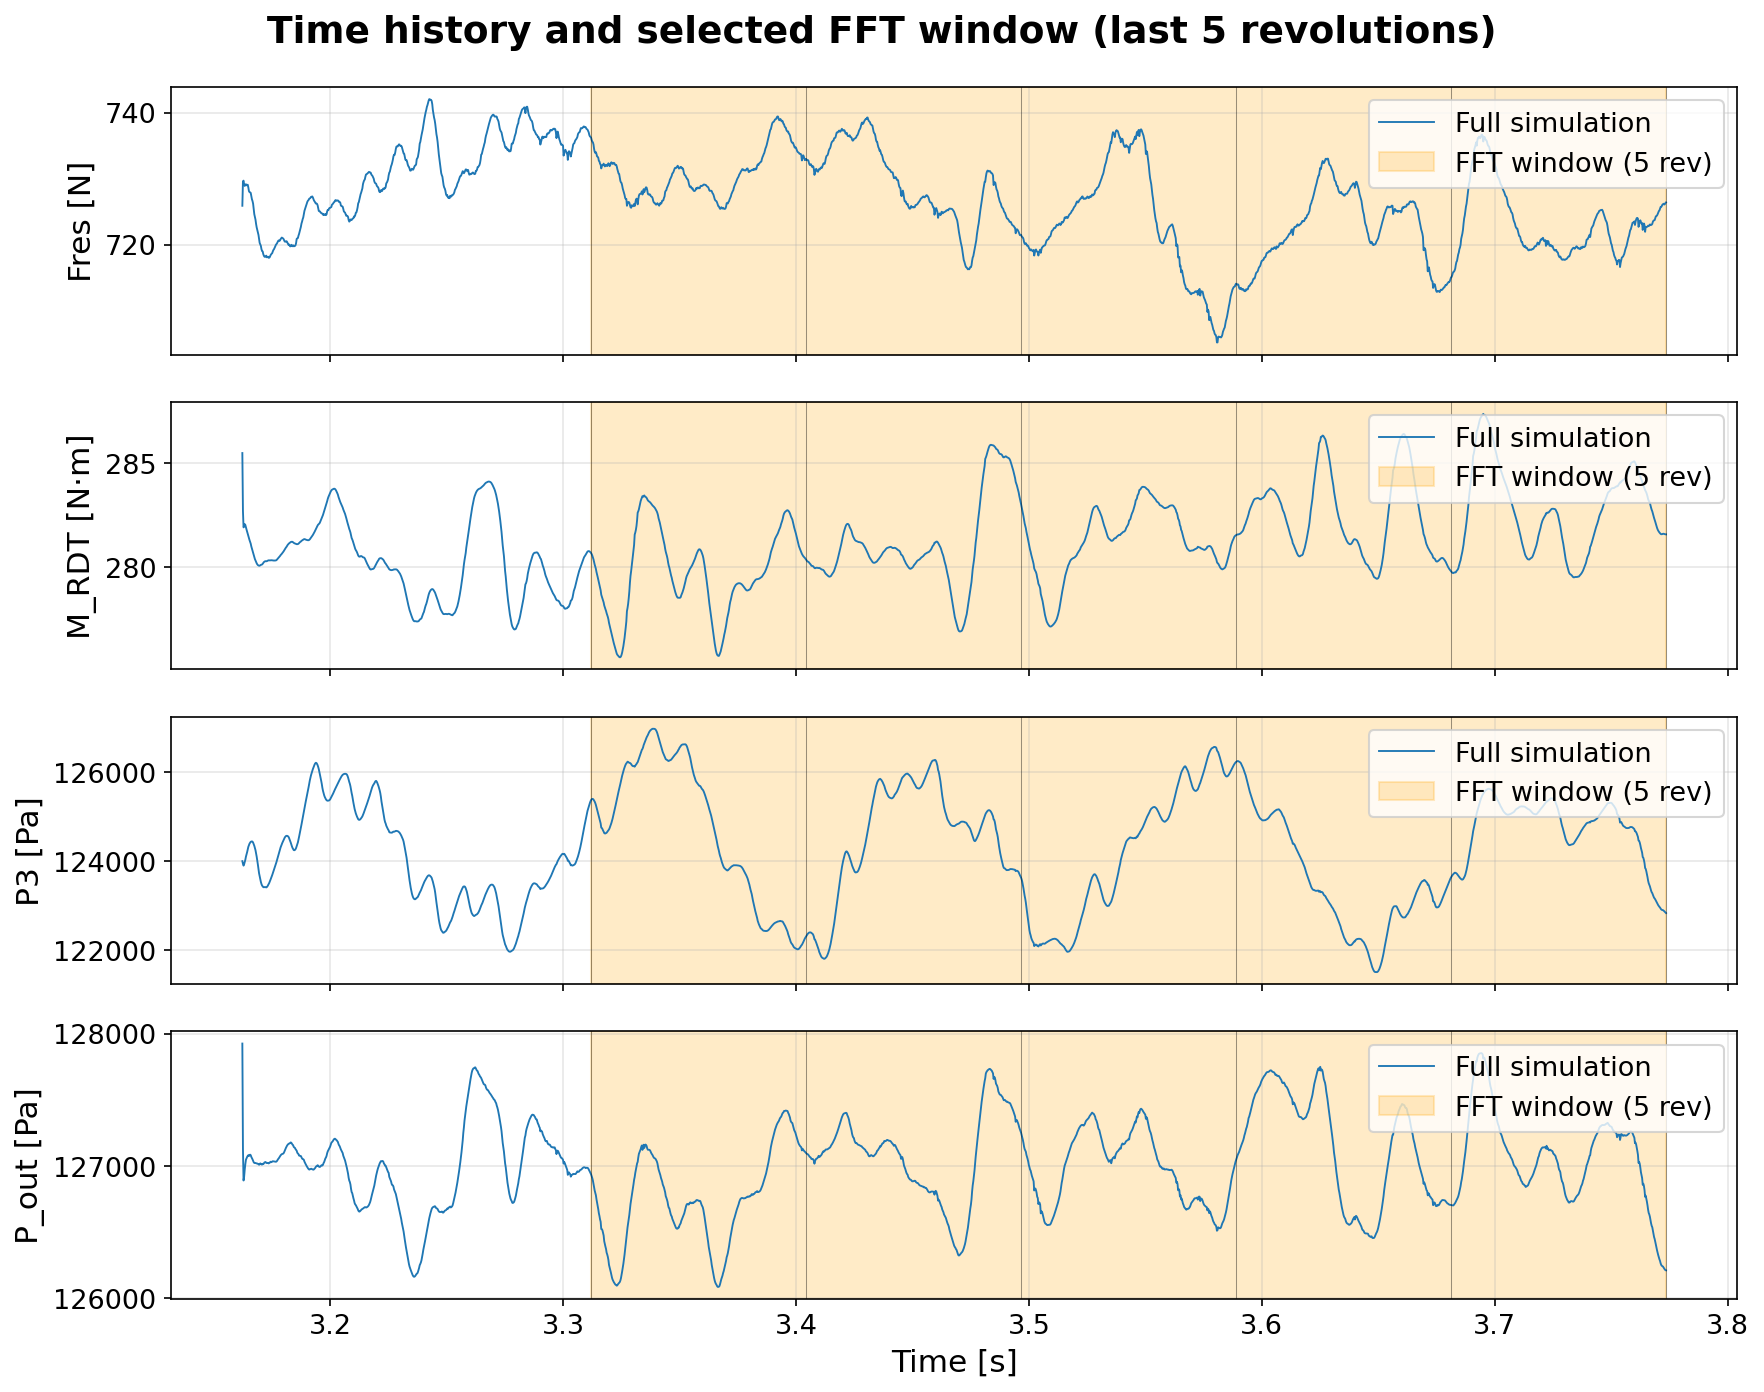
\includegraphics[width=0.95\linewidth]{Figures/FFT/01_timeseries_and_window.png}
\caption{Time histories of four representative monitor signals
($F_{\mathrm{res}}$, $M_{\mathrm{RDT}}$, $P_3$ and
$P_{\mathrm{out}}$) over the exported interval, with the FFT window
(last $5\,T_{\mathrm{rev}}$) shaded.}
\label{fig:timeseries_and_window}
\end{figure}

The phase-folded comparison in
Figure~\ref{fig:periodicity_phase_fold} shows that the five
revolutions within the window do not collapse onto a single curve.
This indicates that the signals carry energy at frequencies below
$f_n$ in addition to the rotor and blade-passing harmonics, which
is consistent with the presence of a once-per-revolution modulation
superimposed on the deterministic blade-passing forcing. The
deviation between revolutions is systematic rather than random,
pointing to a flow-field feature that rotates with the rotor but
does not precisely align with the blade count.

\begin{figure}[H]
\centering
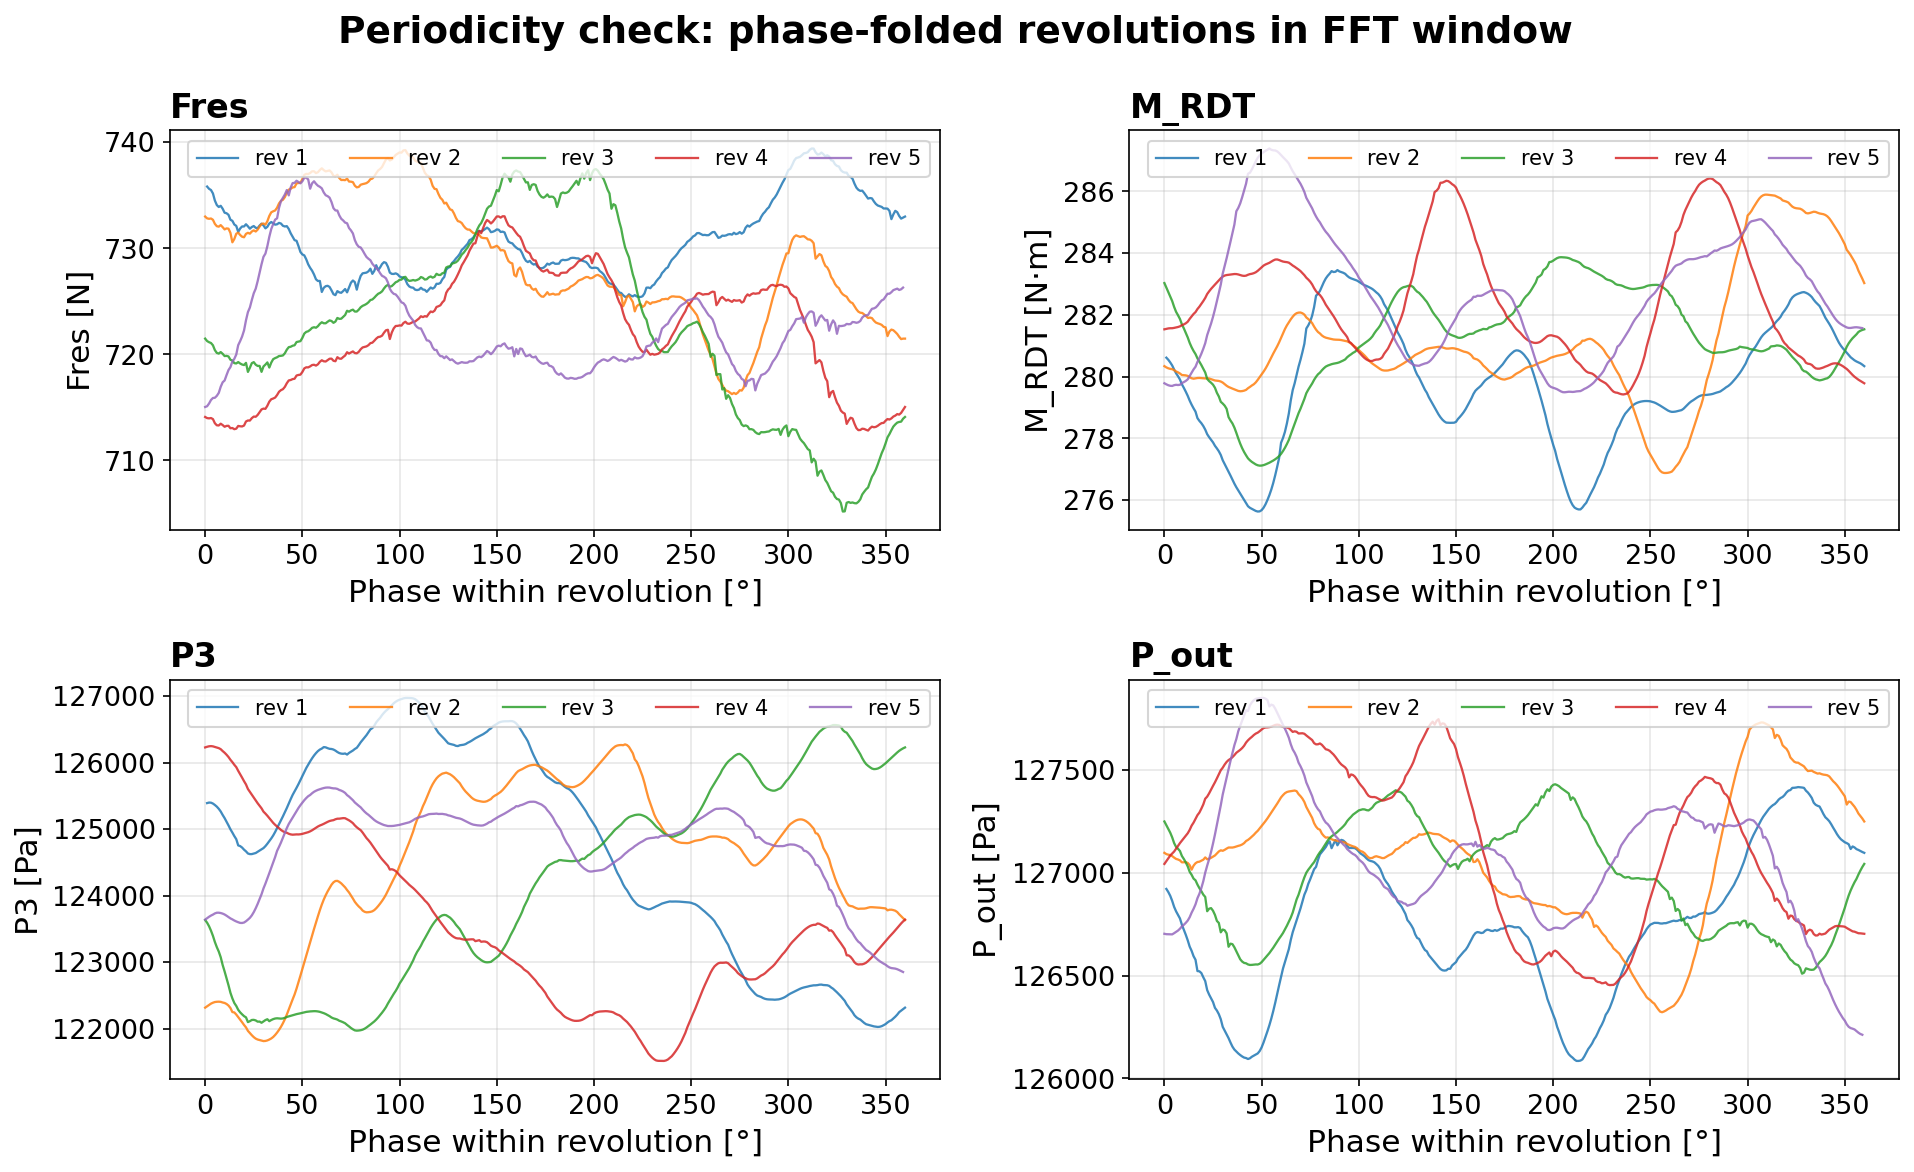
\includegraphics[width=0.95\linewidth]{Figures/FFT/02_periodicity_phase_fold.png}
\caption{Phase-folded time series over the five revolutions in the
FFT window, plotted on a common $0$--$360^\circ$ phase axis. The
lack of collapse onto a single curve indicates content at
frequencies below $f_n$ in addition to the rotor and blade-passing
harmonics.}
\label{fig:periodicity_phase_fold}
\end{figure}

The window robustness test is shown in
Figure~\ref{fig:robustness_5_vs_6}. The spectra computed from the
last five and the last six rotor revolutions are essentially
identical at the characteristic frequencies $f_n$ and
$f_{\mathrm{BPF}}$, and the peak amplitudes agree to within the bin
resolution. The reported amplitudes are therefore not sensitive to
the particular choice of $N_{\mathrm{rev}}$.

\begin{figure}[H]
\centering
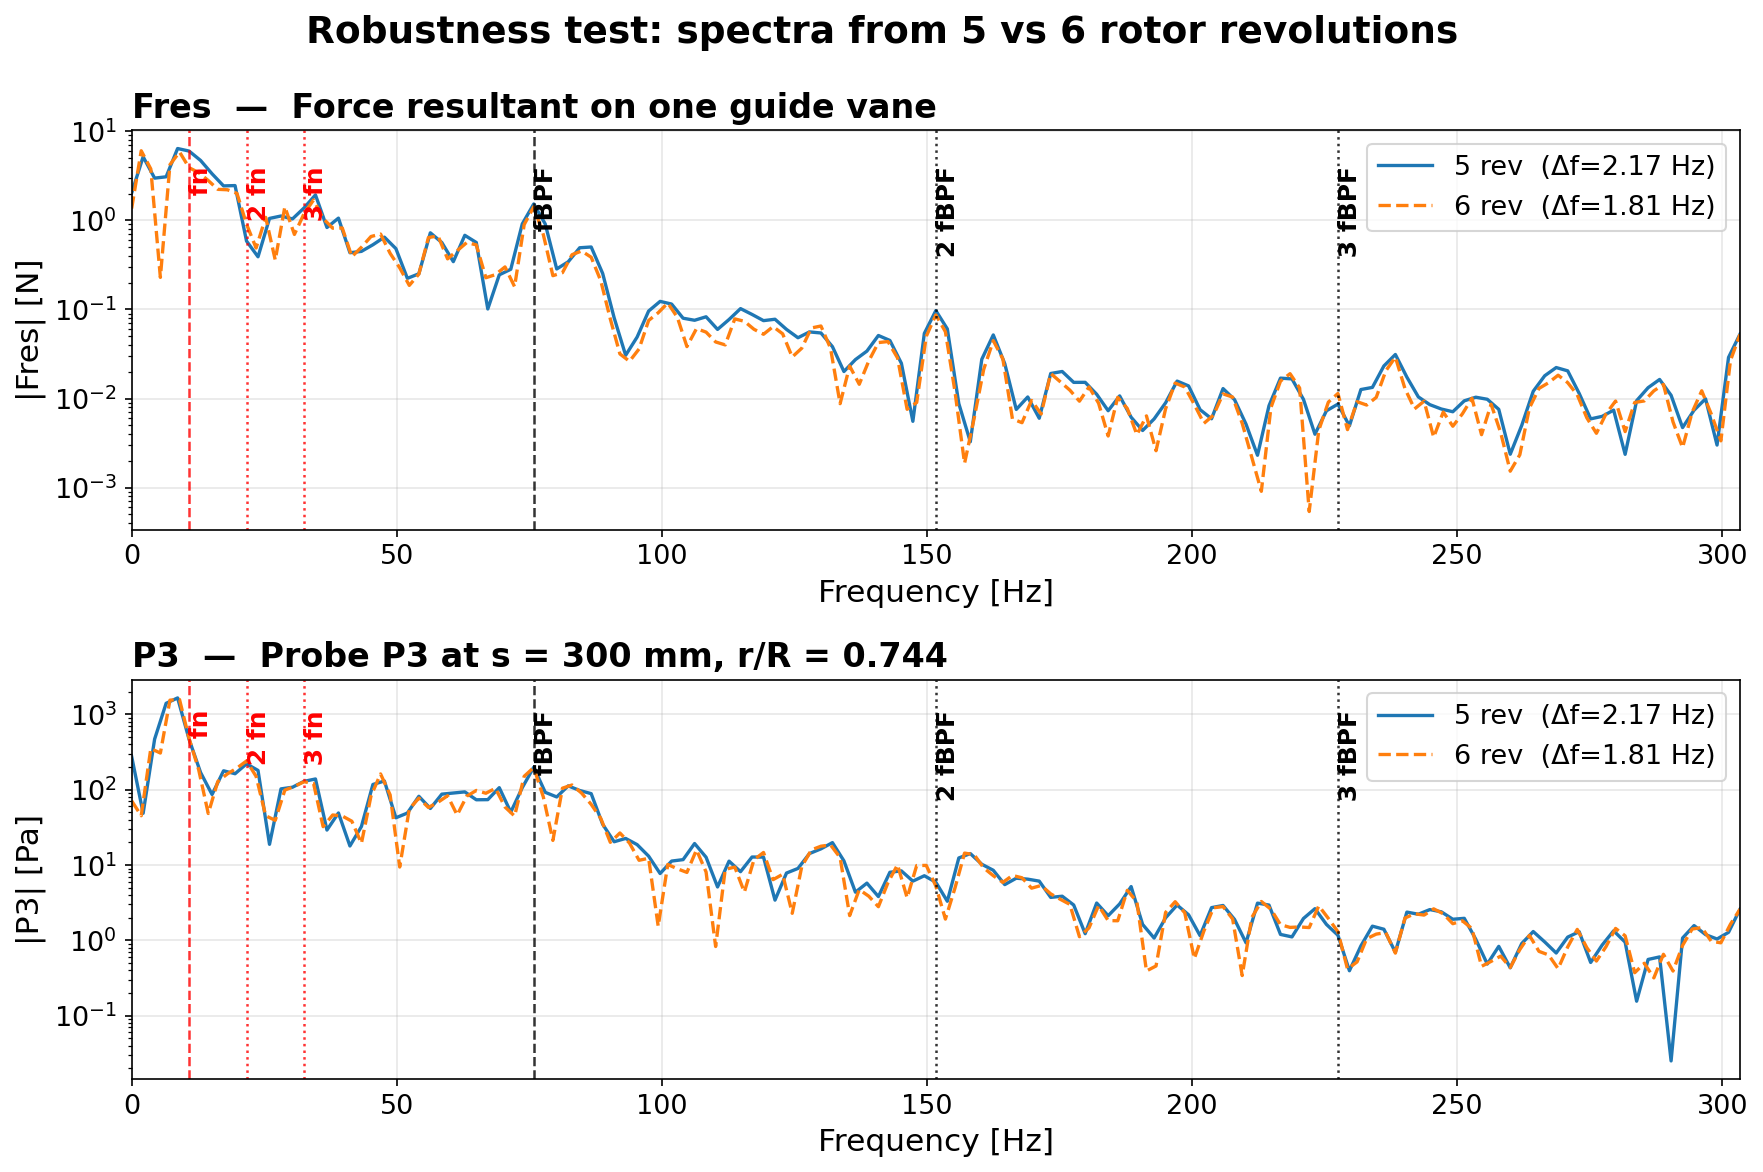
\includegraphics[width=0.95\linewidth]{Figures/FFT/08_robustness_5_vs_6rev.png}
\caption{Robustness of the FFT peak amplitudes to the choice of
analysis window. Spectra from five and six rotor revolutions are
overlaid for $F_{\mathrm{res}}$ and $P_3$.}
\label{fig:robustness_5_vs_6}
\end{figure}

\subsection{Peak amplitudes across all monitor signals}
\label{sec:results-peaks}

Table~\ref{tab:peak_amplitudes} lists the Hanning-windowed peak
amplitudes of all fifteen analysed signals at the two frequencies of
primary interest, $f_n$ and $f_{\mathrm{BPF}}$. The ratio
$A(f_{\mathrm{BPF}})/A(f_n)$ is a compact indicator of which of the
two forcing mechanisms dominates. Values below unity imply that the
once-per-revolution content exceeds the blade-passing content;
values above unity imply the reverse.

\begin{table}[H]
\centering
\small
\caption{Peak amplitudes at the rotor frequency $f_n = 10.83$~Hz
and at the blade passing frequency $f_{\mathrm{BPF}} = 75.83$~Hz for
all monitor signals retained in the analysis. Hanning-windowed FFT
over the last five rotor revolutions.}
\label{tab:peak_amplitudes}
\begin{tabular}{llcccc}
\hline
Label & Description & Unit & $A(f_n)$ & $A(f_{\mathrm{BPF}})$ & Ratio \\ \hline
$F_{\mathrm{res}}$        & Force resultant on GV    & N    & 6.00  & 1.53  & 0.26 \\
$F_x$                      & Force $x$-direction on GV& N    & 4.28  & 0.35  & 0.08 \\
$F_y$                      & Force $y$-direction on GV& N    & 23.5  & 3.39  & 0.14 \\
$F_z$                      & Force $z$-direction on GV& N    & 6.16  & 2.42  & 0.39 \\
$M_{\mathrm{RDT}}$         & Torque about rotation axis (full RDT) & N\,m & 0.101 & 0.089 & 0.88 \\ \hline
$P_{\mathrm{in}}$          & Avg.\ pressure, RDT--GV interface   & Pa & 10.9 & 49.5 & \textbf{4.56} \\
$P_{\mathrm{out}}$         & Avg.\ pressure, downstream of GV    & Pa & 215  & 25.0 & 0.12 \\
$P_{\mathrm{out}}^{\,a}$   & Area-avg.\ pressure downstream of GV & Pa & 175 & 24.2 & 0.14 \\ \hline
$P_{\mathrm{bend}}$        & Pressure at pipe centre before bend & Pa & 32.4 & 26.6 & 0.82 \\ \hline
$P_0$ & Wall probe at $s = 0$~mm    ($r/R = 0.744$) & Pa & 365 & 196  & 0.54 \\
$P_1$ & Wall probe at $s = 100$~mm  ($r/R = 0.744$) & Pa & 576 & 129  & 0.22 \\
$P_2$ & Wall probe at $s = 200$~mm  ($r/R = 0.744$) & Pa & 273 & 57.9 & 0.21 \\
$P_3$ & Wall probe at $s = 300$~mm  ($r/R = 0.744$) & Pa & 468 & 199  & 0.43 \\
$P_4$ & Wall probe at $s = 400$~mm  ($r/R = 0.744$) & Pa & 602 & 85.8 & 0.14 \\
$P_5$ & Wall probe at $s = 500$~mm  ($r/R = 0.744$) & Pa & 322 & 46.0 & 0.14 \\ \hline
\end{tabular}
\end{table}

The cross-signal summary is shown in
Figure~\ref{fig:comparison_fn_vs_fbpf}. Three observations follow
directly from the numbers.

\begin{figure}[H]
\centering
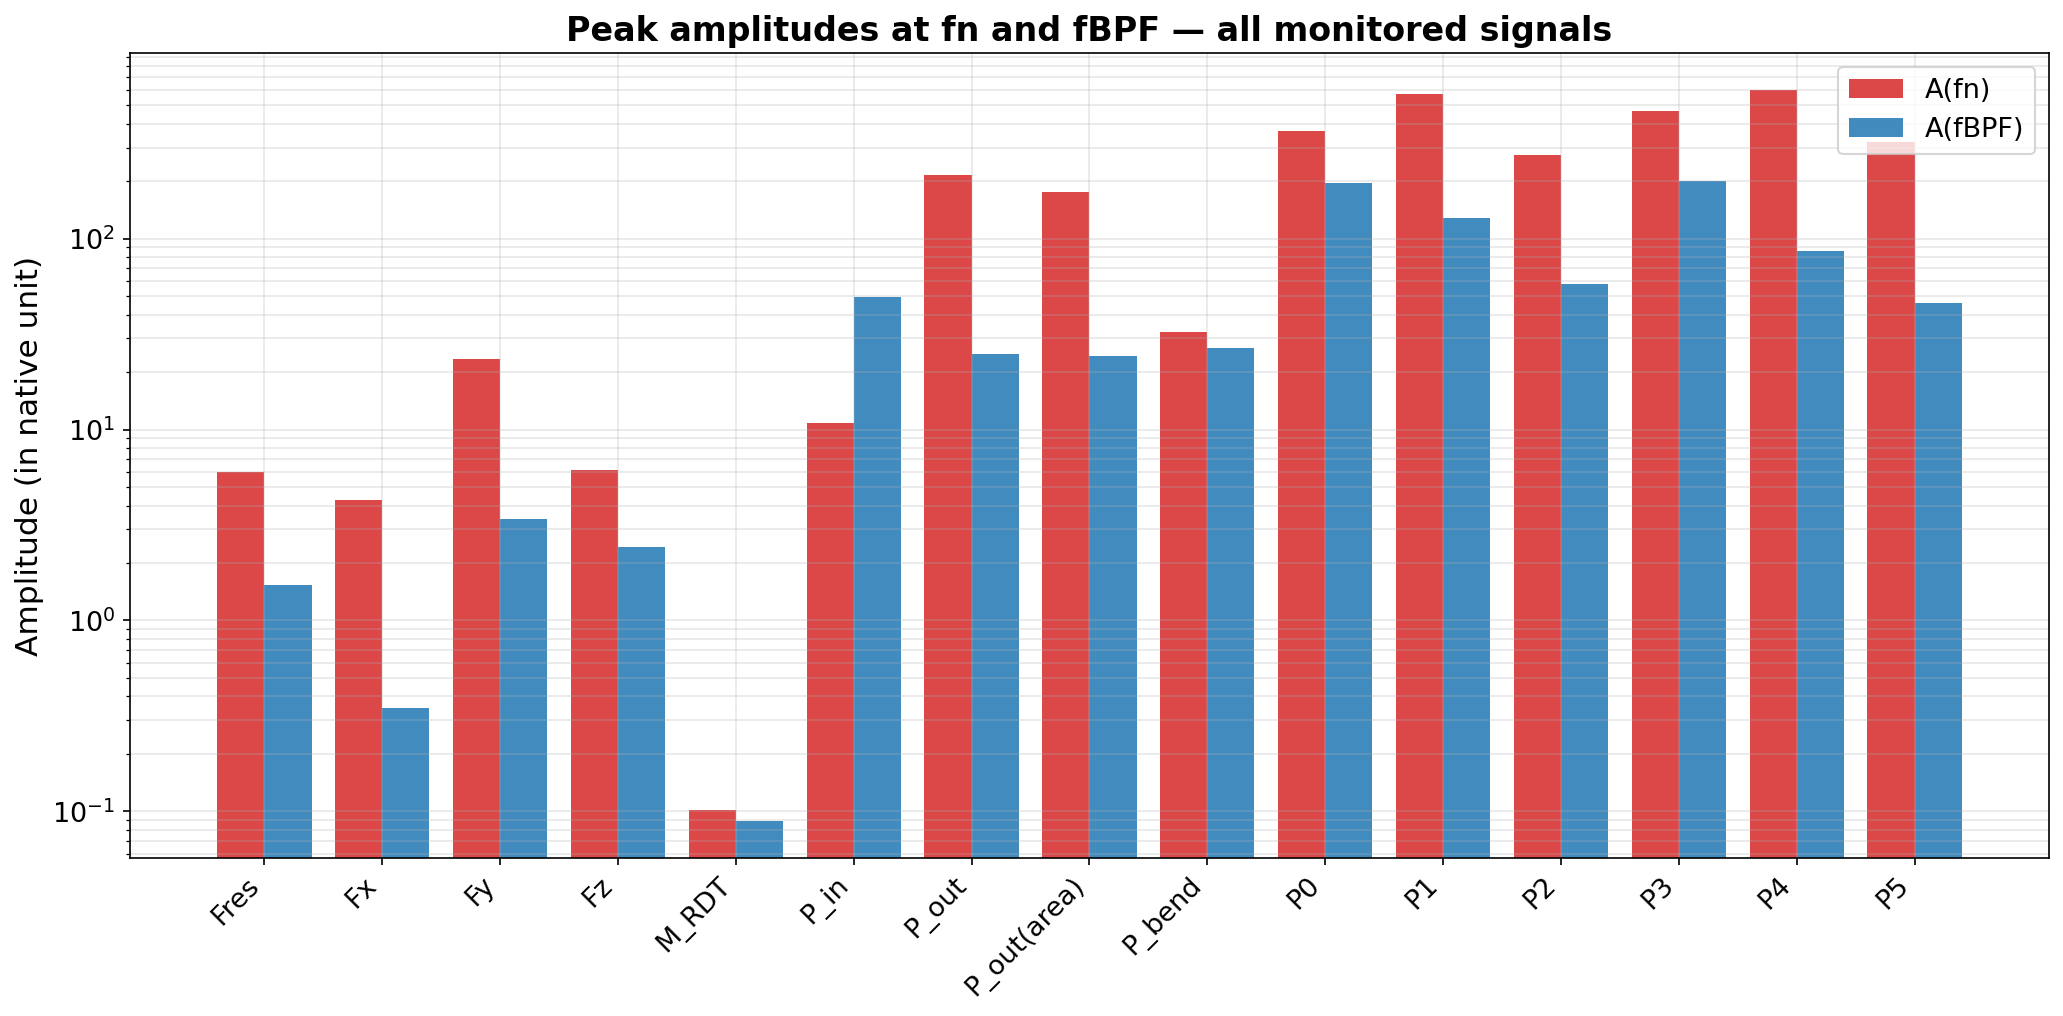
\includegraphics[width=0.95\linewidth]{Figures/FFT/comparison_fn_vs_fBPF_all_signals.png}
\caption{Peak amplitudes at $f_n$ (red) and $f_{\mathrm{BPF}}$
(blue) for all fifteen monitor signals. Amplitudes are plotted in
each signal's native unit on a logarithmic axis. Short labels
follow Table~\ref{tab:monitor-index}.}
\label{fig:comparison_fn_vs_fbpf}
\end{figure}

\paragraph{1. The structural loading on a single guide vane is
dominated by $f_n$, not by $f_{\mathrm{BPF}}$.}
The resultant force $F_{\mathrm{res}}$ has a peak amplitude of
$6.0$~N at $f_n$ but only $1.5$~N at $f_{\mathrm{BPF}}$. Referred
to the mean vane load of approximately $725$~N, the cyclic force
amplitude at $f_{\mathrm{BPF}}$ corresponds to
$1.5/725 \approx 0.21\,\%$ of the mean. This is well below the
$0.5\,\%$ diagnostic threshold for safely operating Francis-type
machines quoted in Section~\ref{sec:rsi-magnitudes}. The larger
$f_n$ amplitude represents a once-per-revolution modulation
consistent with residual azimuthal non-uniformity in the \ac{RDT}
wake.

\paragraph{2. The plane-averaged pressure upstream of the GV row is
the only signal with $f_{\mathrm{BPF}}$ dominance.}
$P_{\mathrm{in}}$ at the \ac{RDT}--\ac{GV} interface has
$A(f_{\mathrm{BPF}})/A(f_n) = 4.56$. This is the expected signature
of the $m=0$ breathing mode predicted by the Tyler--Sofrin theory
for $Z_r = Z_s$ (Section~\ref{sec:rsi-tyler}). The absolute
amplitude is, however, modest. With a nominal head of $H = 5$~m,
the normalised pulsation is
\begin{equation}
    \tilde{p}\tsub{E}
    = \frac{A_p(f_{\mathrm{BPF}})}{\rho g H}
    \approx \frac{49.5}{1000 \cdot 9.81 \cdot 5}
    \approx 1.0\times 10^{-3},
    \label{eq:normalised-pulsation}
\end{equation}
i.e.\ $0.1\,\%$ of $\rho g H$. This is one order of magnitude below
the $1\,\%$ threshold that
Brekke~\cite{brekke,brekke2010} associates with significant
rotor-stator interaction, and two orders of magnitude below the
resonance threshold.

\paragraph{3. The pulsation at $f_{\mathrm{BPF}}$ is attenuated
across the \ac{GV} row.}
Comparing the plane-averaged signals, the amplitude at
$f_{\mathrm{BPF}}$ drops from $49.5$~Pa at $P_{\mathrm{in}}$ to
$25.0$~Pa at $P_{\mathrm{out}}$, a damping factor of approximately
$2$. The area-averaged downstream signal
$P_{\mathrm{out}}^{\,a} = 24.2$~Pa confirms the same order of
magnitude. The \ac{GV} row therefore does not amplify the $m=0$
component of the blade-passing pulsation; it partially attenuates it.

The detailed axial evolution of the wall-pressure pulsation
amplitudes through the \ac{GV} passage is shown in
Figure~\ref{fig:amp_vs_distance_in_GV}. The fundamental $f_n$ and
$f_{\mathrm{BPF}}$ components fluctuate between probes without a
monotonic trend, reflecting the complex spatial structure of the
pulsation field inside the vane passage (a mixture of $m=0$ and
higher-order $m$ modes whose axial phase speeds differ). The
higher harmonics $2 f_{\mathrm{BPF}}$ and $3 f_{\mathrm{BPF}}$ are
one to two orders of magnitude smaller than the fundamental.

\begin{figure}[H]
\centering
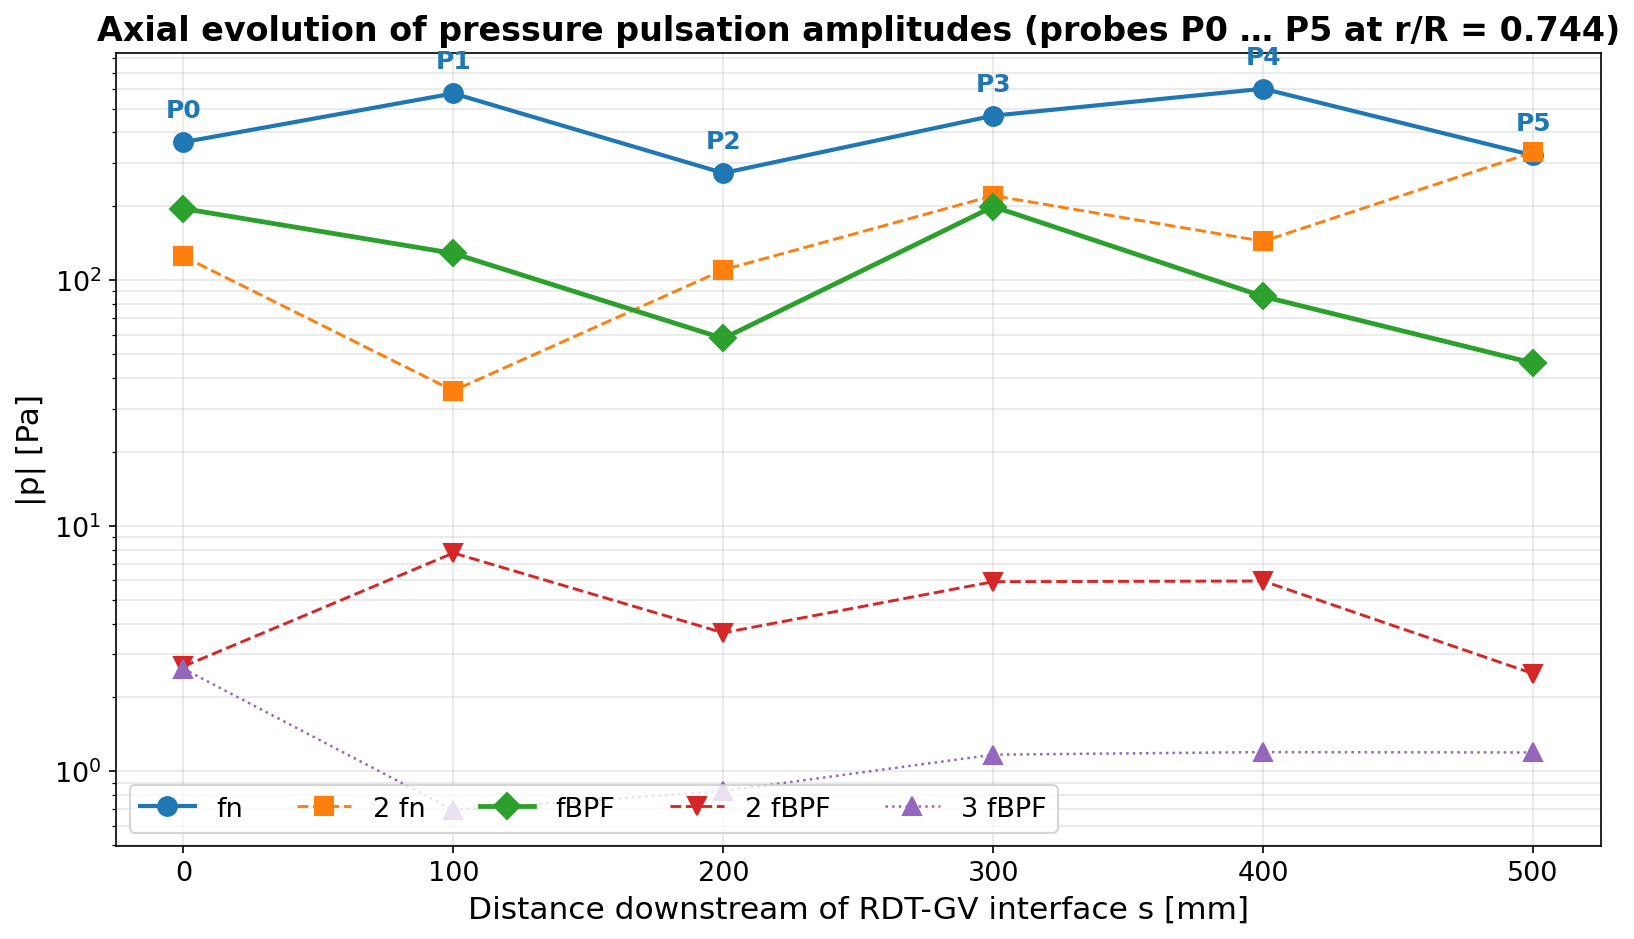
\includegraphics[width=0.9\linewidth]{Figures/FFT/amp_vs_distance_in_GV.png}
\caption{Axial evolution of the wall-pressure pulsation amplitudes
at $r/R = 0.744$ along the \ac{GV} passage, plotted against the
distance $s$ downstream of the \ac{RDT}--\ac{GV} interface.
Labels $P_0\ldots P_5$ correspond to Table~\ref{tab:monitor-index}.}
\label{fig:amp_vs_distance_in_GV}
\end{figure}

Individual spectra for all fifteen signals, including the time
history, statistics summary, spectrum in Hz and spectrum in
$f/f_n$, are provided in Appendix~\ref{app:individual_spectra}.

\subsection{Ring-coherence diagnostic}
\label{sec:results-coherence}

The ring-coherence diagnostic $\mathcal{R}_m(f)$ defined by
Eq.~\eqref{eq:coherence} is computed by dividing the
plane-averaged amplitude $A_{\mathrm{ring}}(f)$ on the downstream
plane by the local wall-pressure amplitude
$A_{\mathrm{loc}}(f)$ at the two representative stations $P_3$
($s=300$~mm) and $P_4$ ($s=400$~mm), which are located immediately
downstream of the \ac{GV} trailing edge region. The resulting
comparison is plotted in Figure~\ref{fig:coherence_check}.

\begin{figure}[H]
\centering
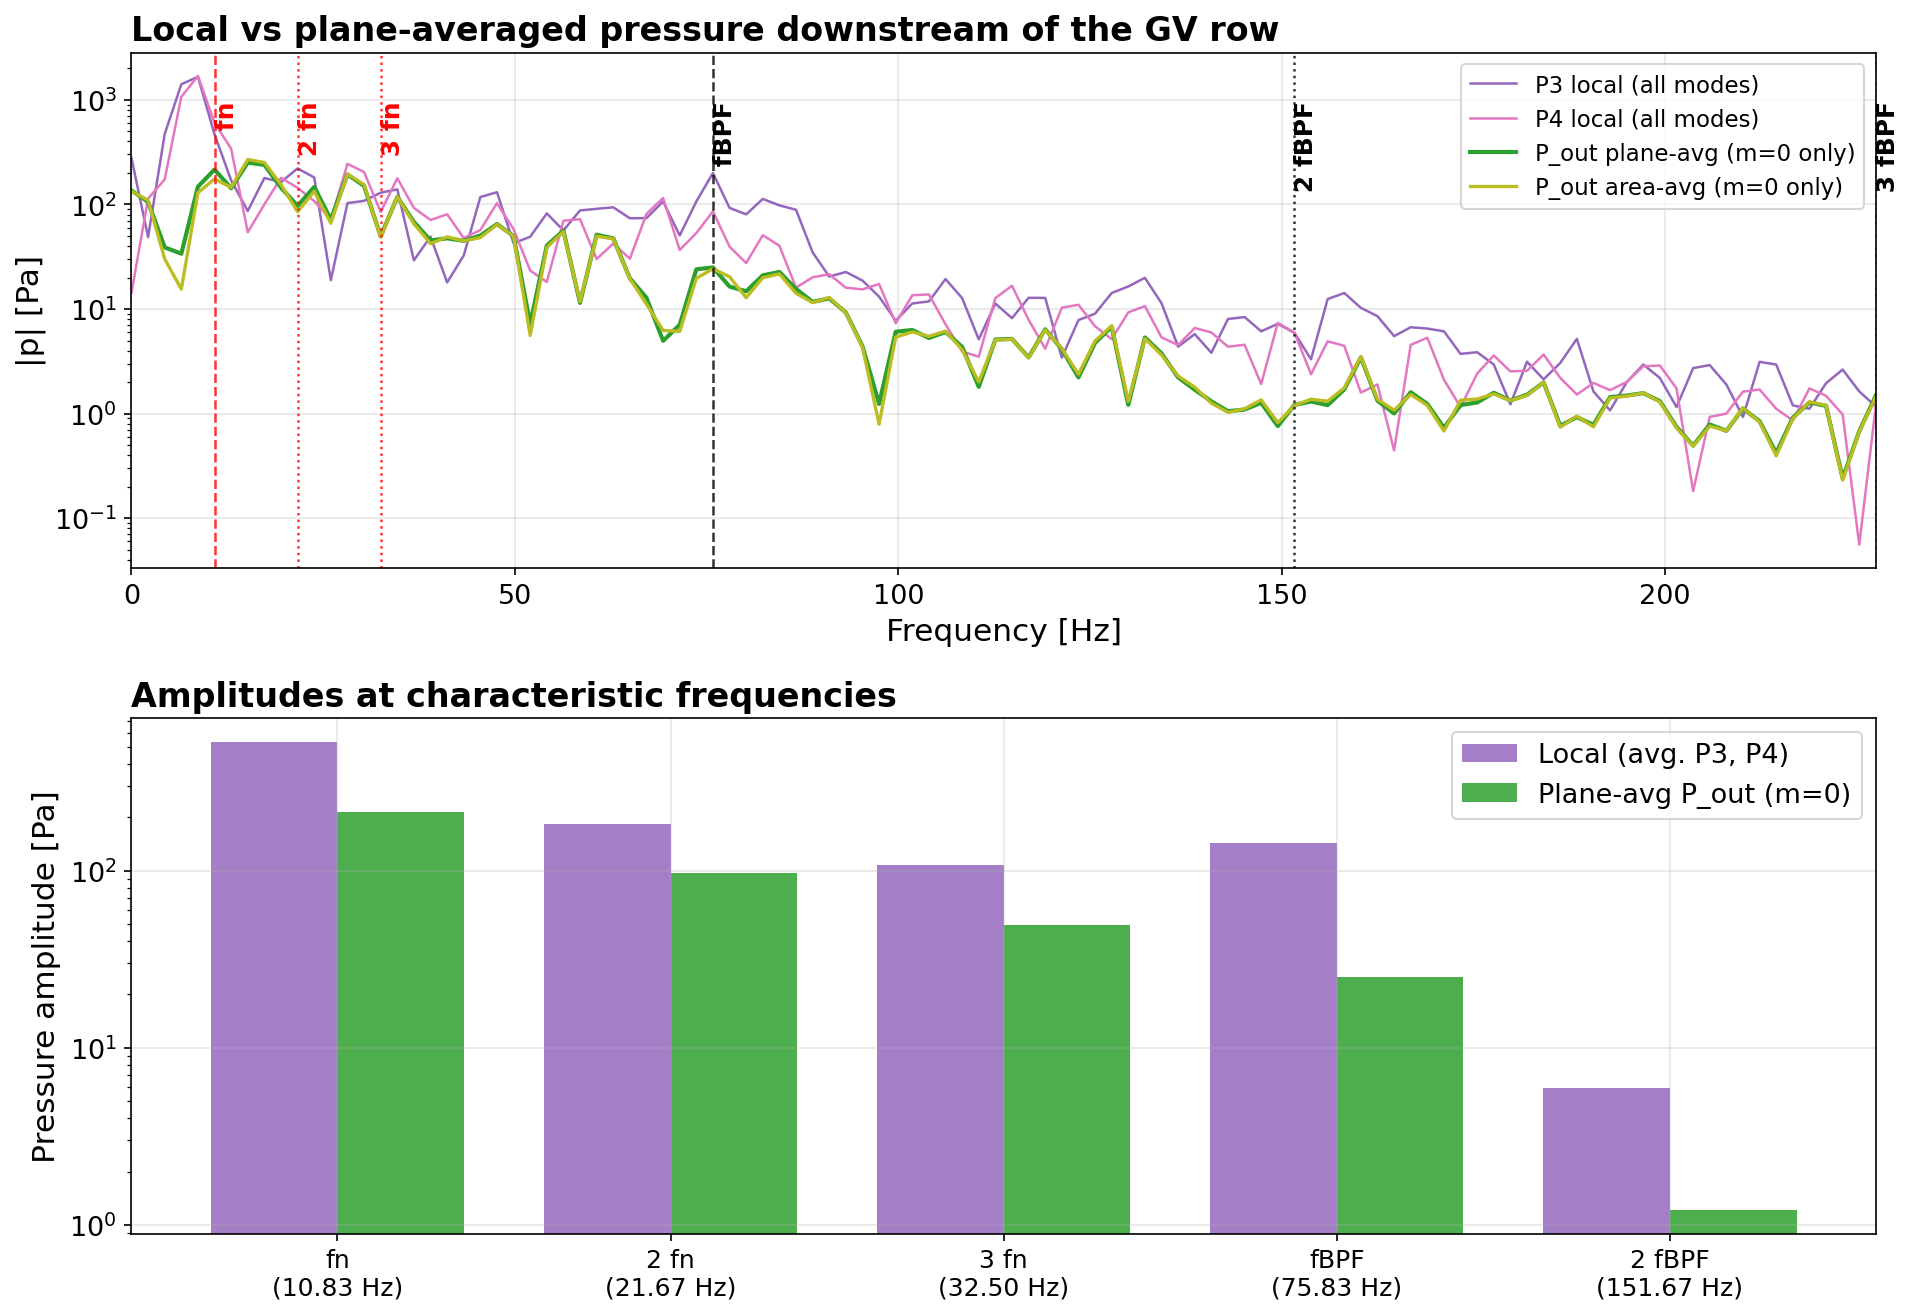
\includegraphics[width=0.95\linewidth]{Figures/FFT/10_coherence_check.png}
\caption{Ring-coherence diagnostic. \emph{Top:} amplitude spectra of
the local wall-pressure signals $P_3$ and $P_4$ (all circumferential
modes) compared with the plane-averaged signals $P_{\mathrm{out}}$
and $P_{\mathrm{out}}^{\,a}$ (only the $m=0$ mode).
\emph{Bottom:} local and plane-averaged amplitudes at the
characteristic frequencies.}
\label{fig:coherence_check}
\end{figure}

At the blade passing frequency the numerical values are
\begin{align}
    A_{\mathrm{loc}}(f_{\mathrm{BPF}})
      &\approx 143~\mathrm{Pa} \qquad
        (\text{average of } P_3 \text{ and } P_4), \\
    A_{\mathrm{ring}}(f_{\mathrm{BPF}})
      &\approx 25~\mathrm{Pa},
\end{align}
so that
\begin{equation}
    \mathcal{R}_m(f_{\mathrm{BPF}}) \;\approx\; 0.17.
    \label{eq:coherence-value}
\end{equation}
The same diagnostic at $f_n$ gives
$\mathcal{R}_m(f_n) \approx 0.40$. Both values are much smaller than
unity. The pulsation field at $f_{\mathrm{BPF}}$ in the present
simulation is therefore \emph{not} dominated by the axisymmetric
breathing mode that the Tyler--Sofrin analysis predicts for
$Z_r = Z_s = 7$.

This is a non-trivial finding. The mode-order prediction of
Eq.~\eqref{eq:mmin} is based on the assumption that the rotor
produces a perfectly $Z_r$-fold azimuthally symmetric wake. In the
present geometry this assumption is violated for at least two
reasons. First, the \ac{RDT} inflow field contains a small
non-uniform radial component that breaks the $Z_r$-fold symmetry,
as reflected in the residual once-per-revolution variation observed
in the phase-folded time series
(Figure~\ref{fig:periodicity_phase_fold}). Second, the numerical
wake is not identical between blades at the discretisation level
used here. The combined effect is that the coherent $m=0$ content
represents only about $17\,\%$ of the total pulsation at
$f_{\mathrm{BPF}}$ in this simulation, with the remainder
distributed in spinning modes $|m|\geq 1$ that cancel in plane
averaging.

\section{Discussion}
\label{sec:results-fft-discussion}

\subsection{Summary of the quantitative findings}
\label{sec:results-fft-summary}

\begin{itemize}
  \item The peak force amplitude at $f_{\mathrm{BPF}}$ on the
        monitored guide vane is $1.5$~N on a mean load of
        $725$~N, i.e.\ $0.21\,\%$ of the mean. This is below the
        $0.5\,\%$ threshold associated with safely operating
        hydraulic machines (Section~\ref{sec:rsi-magnitudes}).
  \item The normalised pressure pulsation at $f_{\mathrm{BPF}}$ on
        the upstream plane is $0.1\,\%$ of $\rho g H$, one order of
        magnitude below the $1\,\%$ threshold
        of~\cite{brekke,brekke2010} for the onset of significant
        rotor-stator interaction.
  \item The ring-coherence diagnostic gives
        $\mathcal{R}_m(f_{\mathrm{BPF}}) \approx 0.17$, showing
        that the axisymmetric breathing mode predicted by
        Tyler--Sofrin theory for $Z_r = Z_s = 7$ accounts for only
        about one-sixth of the local pulsation at
        $f_{\mathrm{BPF}}$.
  \item The \ac{GV} row attenuates rather than amplifies the $m=0$
        content between the upstream and downstream planes,
        reducing $A(f_{\mathrm{BPF}})$ from $49.5$~Pa at
        $P_{\mathrm{in}}$ to $25.0$~Pa at $P_{\mathrm{out}}$.
\end{itemize}

Taken together, these results indicate that the baseline
$Z_r = Z_s = 7$ configuration does not exhibit a structurally or
hydraulically significant rotor-stator resonance in the present
transient simulation at the nominal operating point.

\subsection{Caveats in the interpretation}
\label{sec:results-fft-caveats}

\paragraph{The present simulation does not include structural
coupling.} Resonance in the strict sense requires an excitation
frequency to approach a structural or acoustic natural frequency of
the system. No modal analysis of the guide vane has been performed
in this work. The statement that the cyclic force amplitude is
below a fatigue-critical level therefore holds under the assumption
that the lowest wet natural frequency of the \ac{GV} is well
separated from $f_{\mathrm{BPF}} = 75.83$~Hz and its low harmonics.
A finite-element modal analysis of the selected final design,
including the added-mass effect of the surrounding
water~\cite{valentin2015}, is recommended as a separate
verification step (Chapter~\ref{ch:future-work}).

\paragraph{The absence of a dominant breathing mode in this
simulation does not invalidate the classical design guideline.}
The Tyler--Sofrin~\cite{tyler1962} mode-order relation
(Eq.~\eqref{eq:tyler_sofrin}) is independent of the wake amplitude.
It only states that for $Z_r = Z_s$, the spatial mode of lowest
circumferential order at $f_{\mathrm{BPF}}$ is $m_{\min} = 0$. If
the rotor wake is, for any reason, more closely $Z_r$-fold
symmetric than in the present simulation --- for example due to a
different mesh topology, finer discretisation, a different inflow
condition, or an operational shift that makes the inflow more
uniform --- the $m=0$ content will grow, and the coherent ring
loading at $f_{\mathrm{BPF}}$ will increase accordingly. The recent
results of Nduwayezu et al.~\cite{nduwayezu2021} explicitly
demonstrate this sensitivity for reversible pump-turbines: the
vaneless-space pressure pulsation amplitude was observed to change
systematically with the runner blade number for otherwise identical
operating conditions. The classical design guideline --- expressed
consistently in Brekke~\cite{brekke,brekke2010},
Egusquiza~et~al.~\cite{egusquiza2006} and
Tanaka~\cite{tanaka2011} --- that $Z_r$ and $Z_s$ should be chosen
so that low-order spatial modes are avoided at the harmonics of
concern therefore remains valid, regardless of the absence of
resonance observed here.

\subsection{Implications for the selection of $Z_s$}
\label{sec:results-fft-implications}

The spectral analysis has two distinct roles in the overall thesis
argument:
\begin{enumerate}
  \item It demonstrates that the transient \ac{RDT}--\ac{GV}--duct
        simulation is numerically well-behaved at the nominal
        operating point, and that the pulsation amplitudes produced
        by the setup are physically reasonable and below industrial
        concern thresholds. This provides the verification needed
        for interpreting the hydraulic (steady-state) screening
        results reported in Chapter~\ref{ch:results-hydraulic} with
        confidence that the associated transient forcing levels are
        acceptable.
  \item It tests, in the specific \ac{RDT}--\ac{GV} geometry of this
        project, the classical theoretical concern that
        $Z_r = Z_s$ should be avoided. The result is nuanced: the
        worst-case $m=0$ pulsation predicted by the theory is
        present but does not dominate, and the pulsation levels
        remain well below the thresholds
        from~\cite{brekke,brekke2010}.
\end{enumerate}

The final \ac{GV} design recommended in this thesis is nevertheless
taken from the subset of the 24-case design matrix with
$Z_s \neq Z_r$. This choice follows the conservative interpretation
of the classical guideline: the absence of dominant $m=0$ content
in the baseline simulation depends on a specific combination of
wake asymmetry and numerical discretisation that cannot be
guaranteed for every operating point or every manufactured rotor.
Choosing $Z_s \neq Z_r$ removes the worst-case breathing mode from
the mode-order spectrum altogether and is therefore the robust
choice, consistent with the recommendations
of~\cite{brekke,brekke2010,nduwayezu2021}. Among the two non-equal
options in the design matrix, $Z_s \in \{5, 6\}$, the final
selection is made on the basis of the hydraulic metrics discussed
in Chapter~\ref{ch:results-hydraulic}.

\subsection{Summary of the spectral analysis}
\label{sec:results-fft-summary2}

The transient simulation of the baseline \ac{RDT}--\ac{GV}
configuration with $Z_r = Z_s = 7$ at $n = 650$~rpm shows
blade-passing pulsation amplitudes that are an order of magnitude
below the thresholds associated with significant rotor-stator
interaction. The ring-coherence diagnostic quantifies the
contribution of the axisymmetric breathing mode to the
blade-passing pulsation at approximately $17\,\%$, confirming that
the worst-case $m=0$ scenario predicted by the Tyler--Sofrin theory
for equal blade counts is not fully realised in this specific
configuration. At the same time, the theoretical concern that
motivates the avoidance of $Z_r = Z_s$ remains valid for the final
design selection, as the margin between the observed pulsation
levels and structural thresholds depends on details of the inflow
symmetry that cannot be guaranteed in all operating conditions. The
final \ac{GV} design is therefore selected from the
$Z_s \neq Z_r$ subset of the design matrix.


% ======================================================================
% APPENDIX — Individual monitor-signal spectra
% Place in e.g. appendix/Appendix-G.tex
% ======================================================================

\chapter{Individual monitor-signal spectra from the FFT analysis}
\label{app:individual_spectra}

This appendix contains the individual FFT results for each of the
fifteen monitor signals defined in Table~\ref{tab:monitor-index}.
Each figure shows:
(i) the raw time history with the FFT window highlighted in red;
(ii) a statistics and peak-amplitude summary;
(iii) the amplitude spectrum in Hz up to approximately
$5\,f_{\mathrm{BPF}}$ with rotor and blade-passing harmonics marked;
and (iv) the amplitude spectrum normalised to $f/f_n$ up to
$30\,f_n$.

% ----- Group A: forces on one guide vane -------------------------

\section*{Group A — Forces on one guide vane}

\begin{figure}[H]\centering
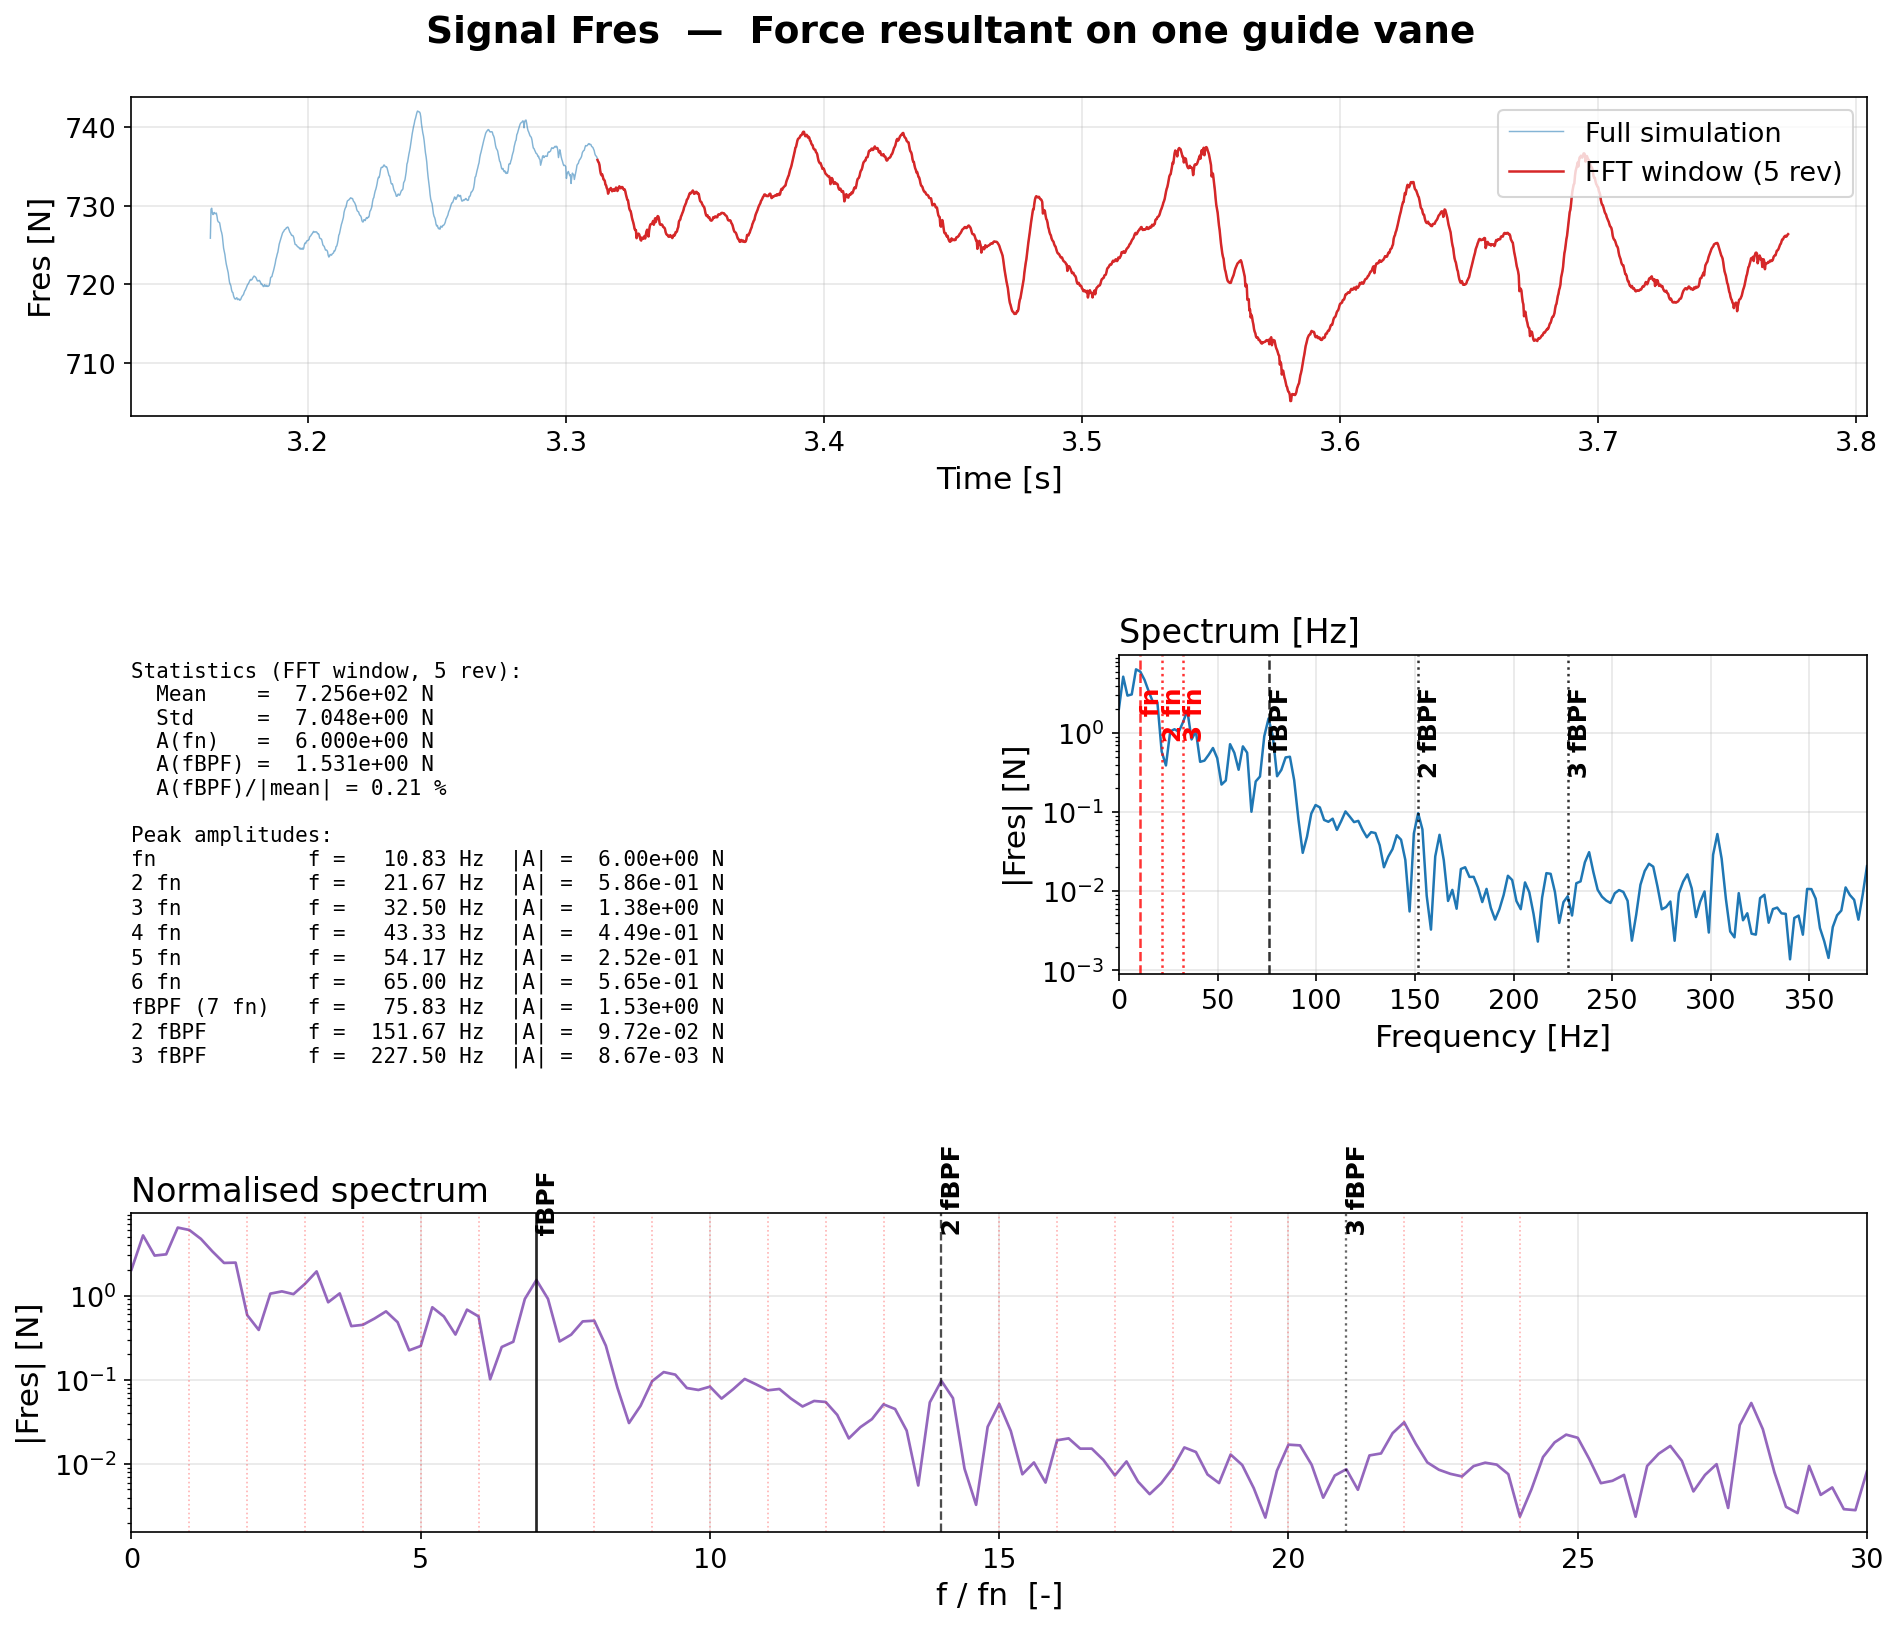
\includegraphics[width=0.95\linewidth]{Figures/FFT/signal_Fres.png}
\caption{$F_{\mathrm{res}}$ — Resultant force on one guide vane.}
\end{figure}

\begin{figure}[H]\centering
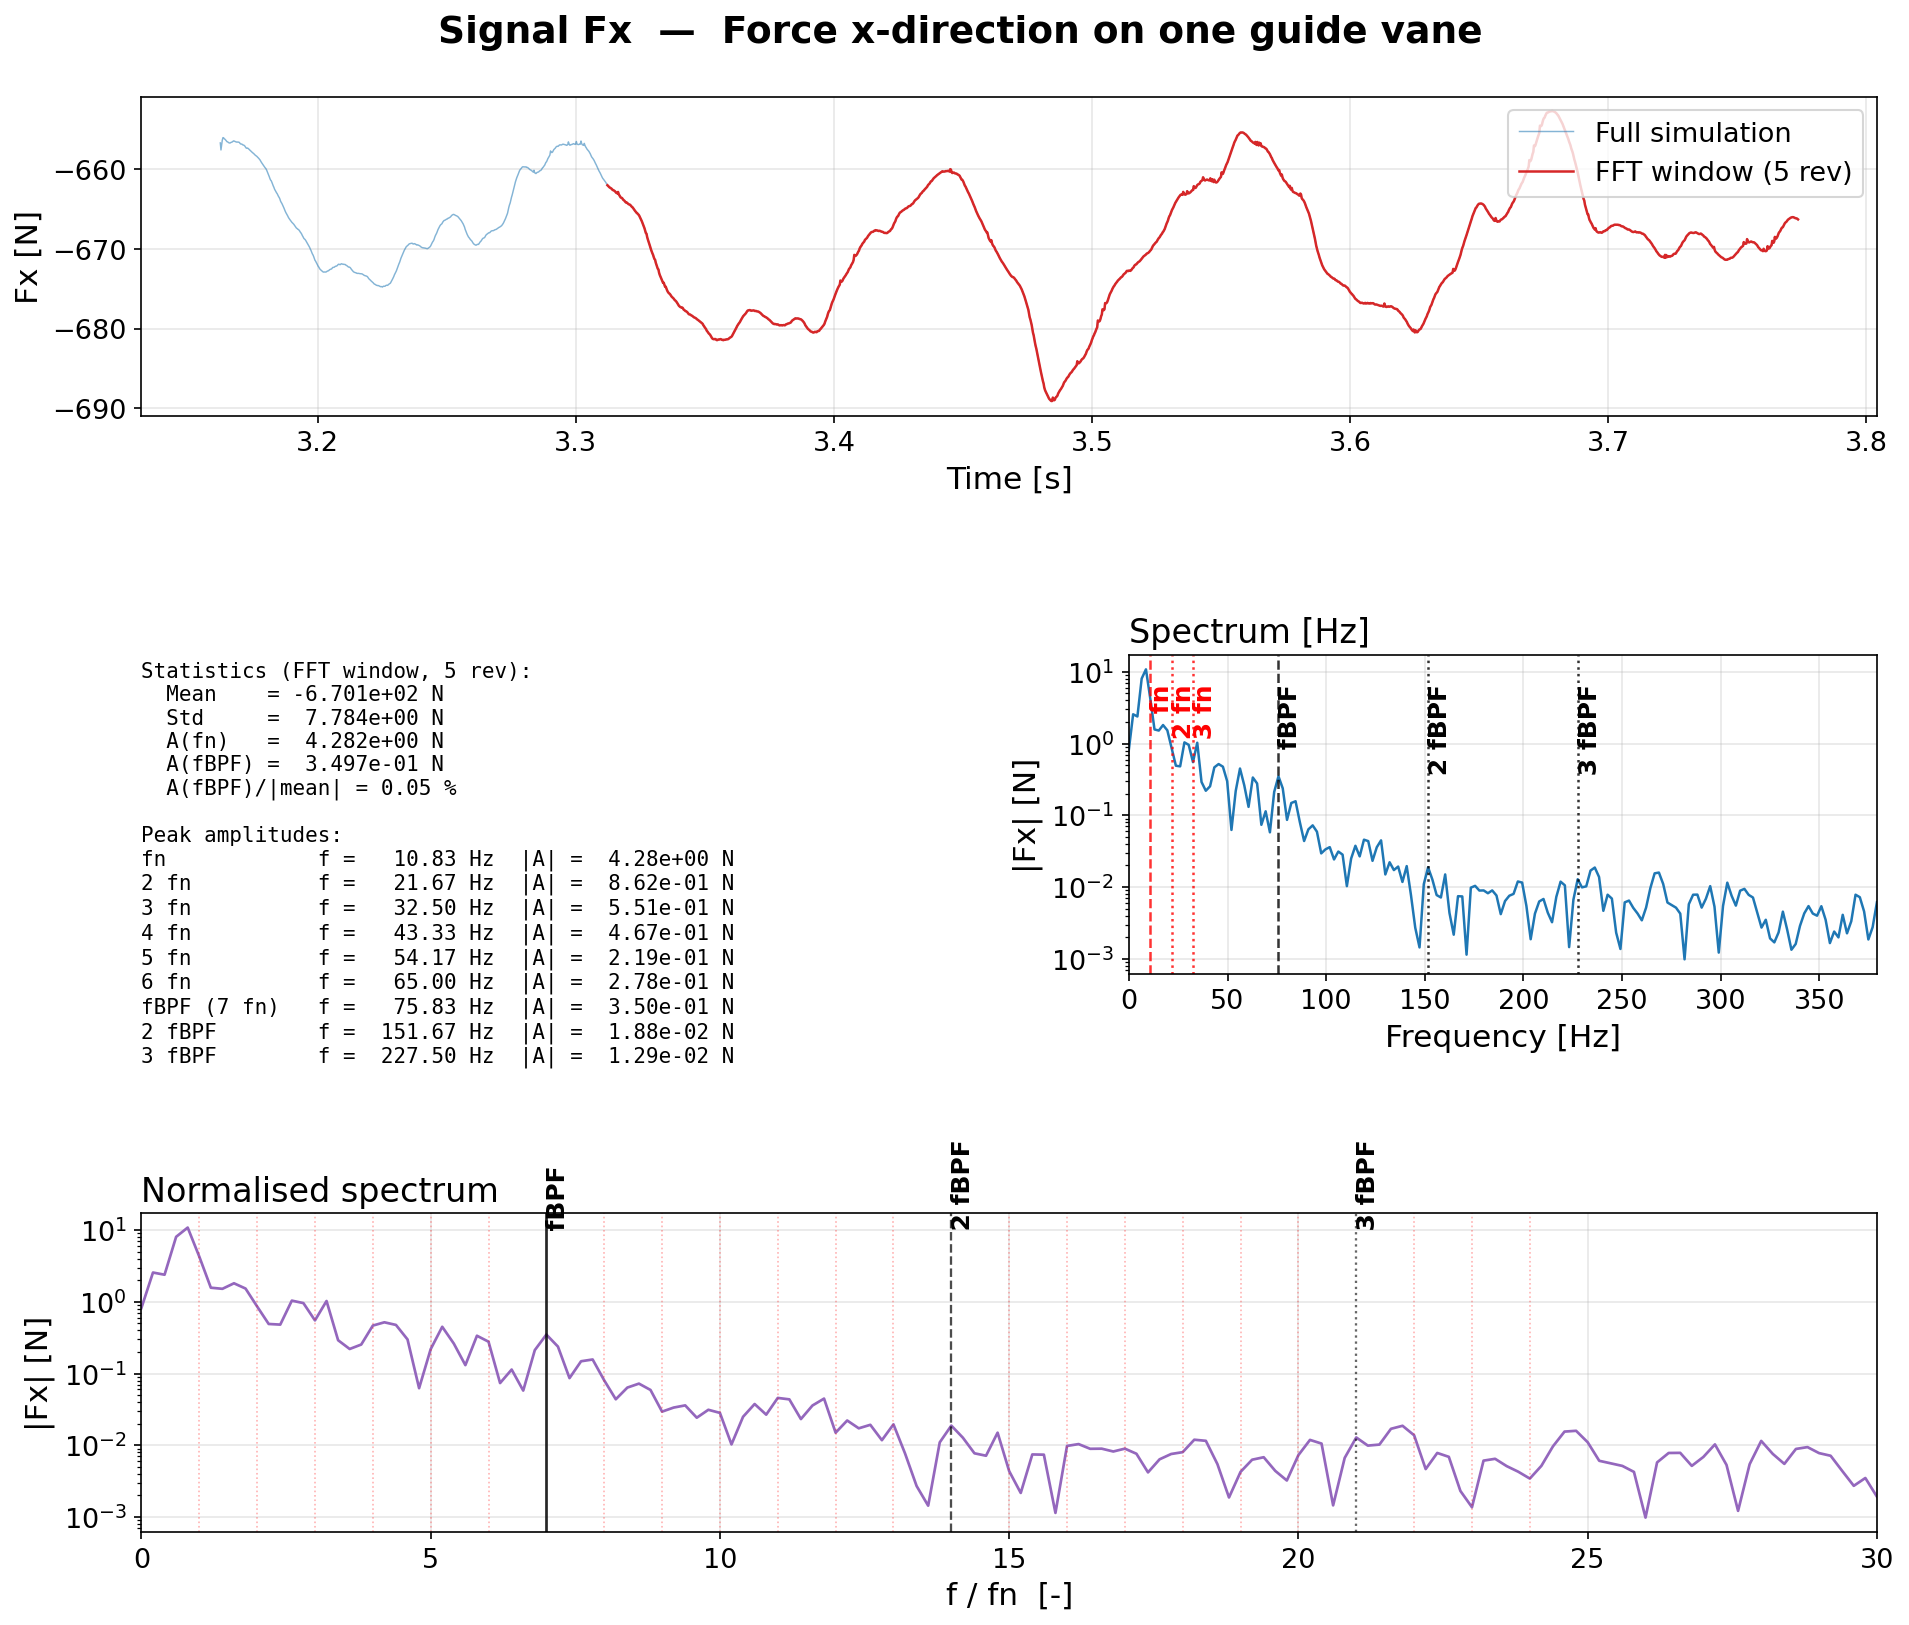
\includegraphics[width=0.95\linewidth]{Figures/FFT/signal_Fx.png}
\caption{$F_x$ — Force $x$-direction on one guide vane.}
\end{figure}

\begin{figure}[H]\centering
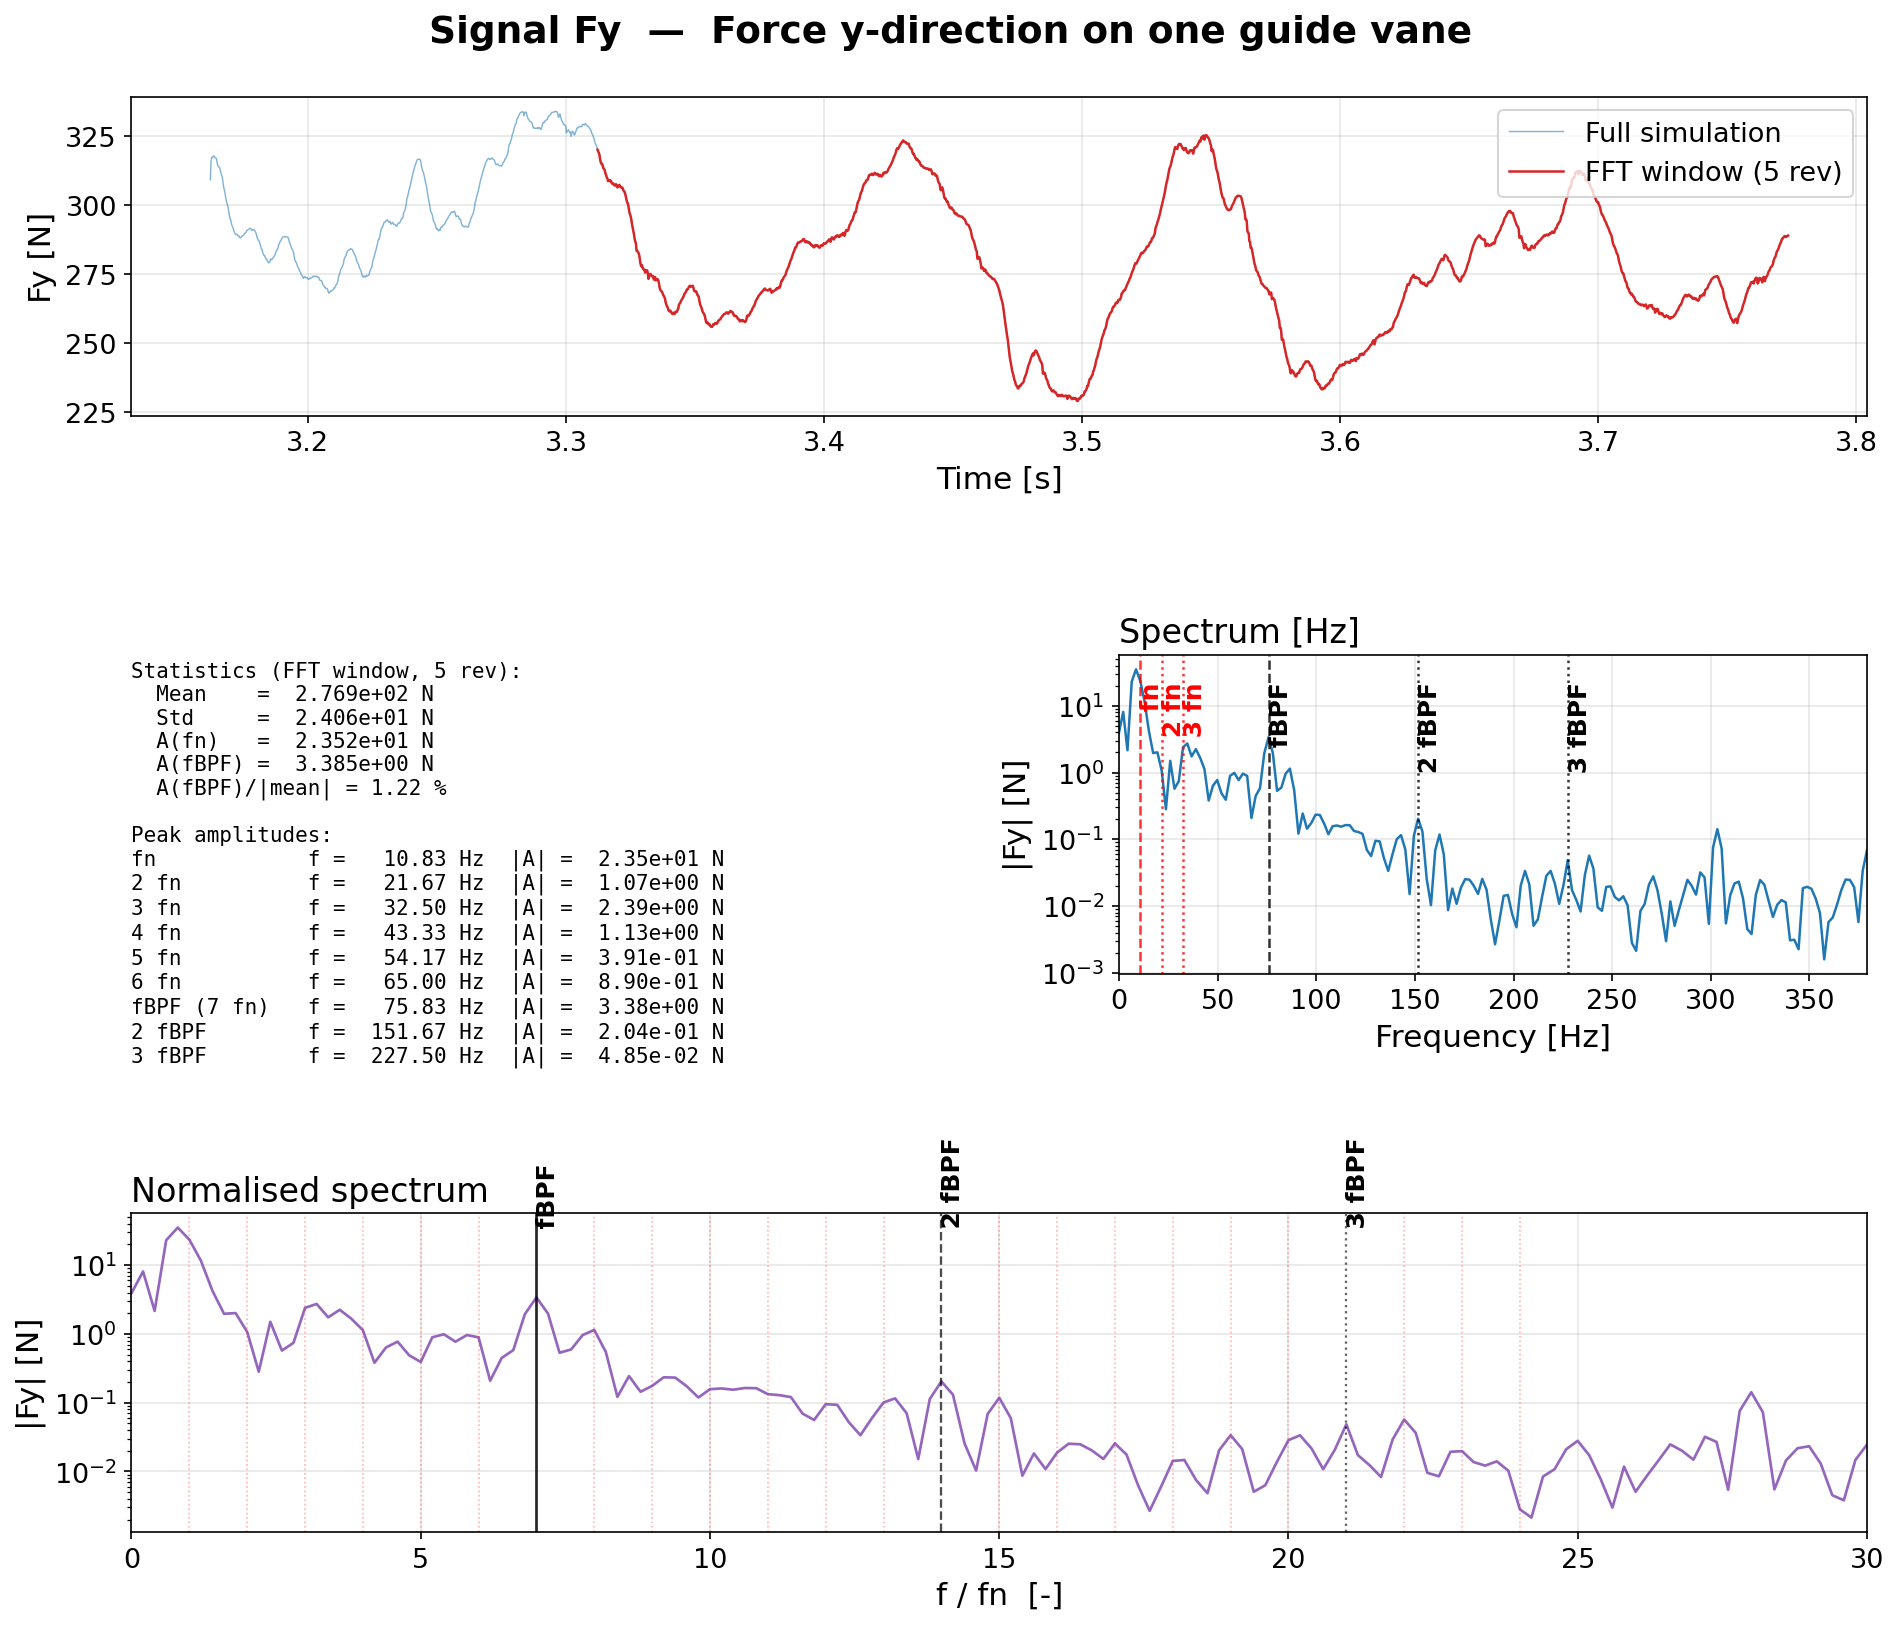
\includegraphics[width=0.95\linewidth]{Figures/FFT/signal_Fy.png}
\caption{$F_y$ — Force $y$-direction on one guide vane.}
\end{figure}

\begin{figure}[H]\centering
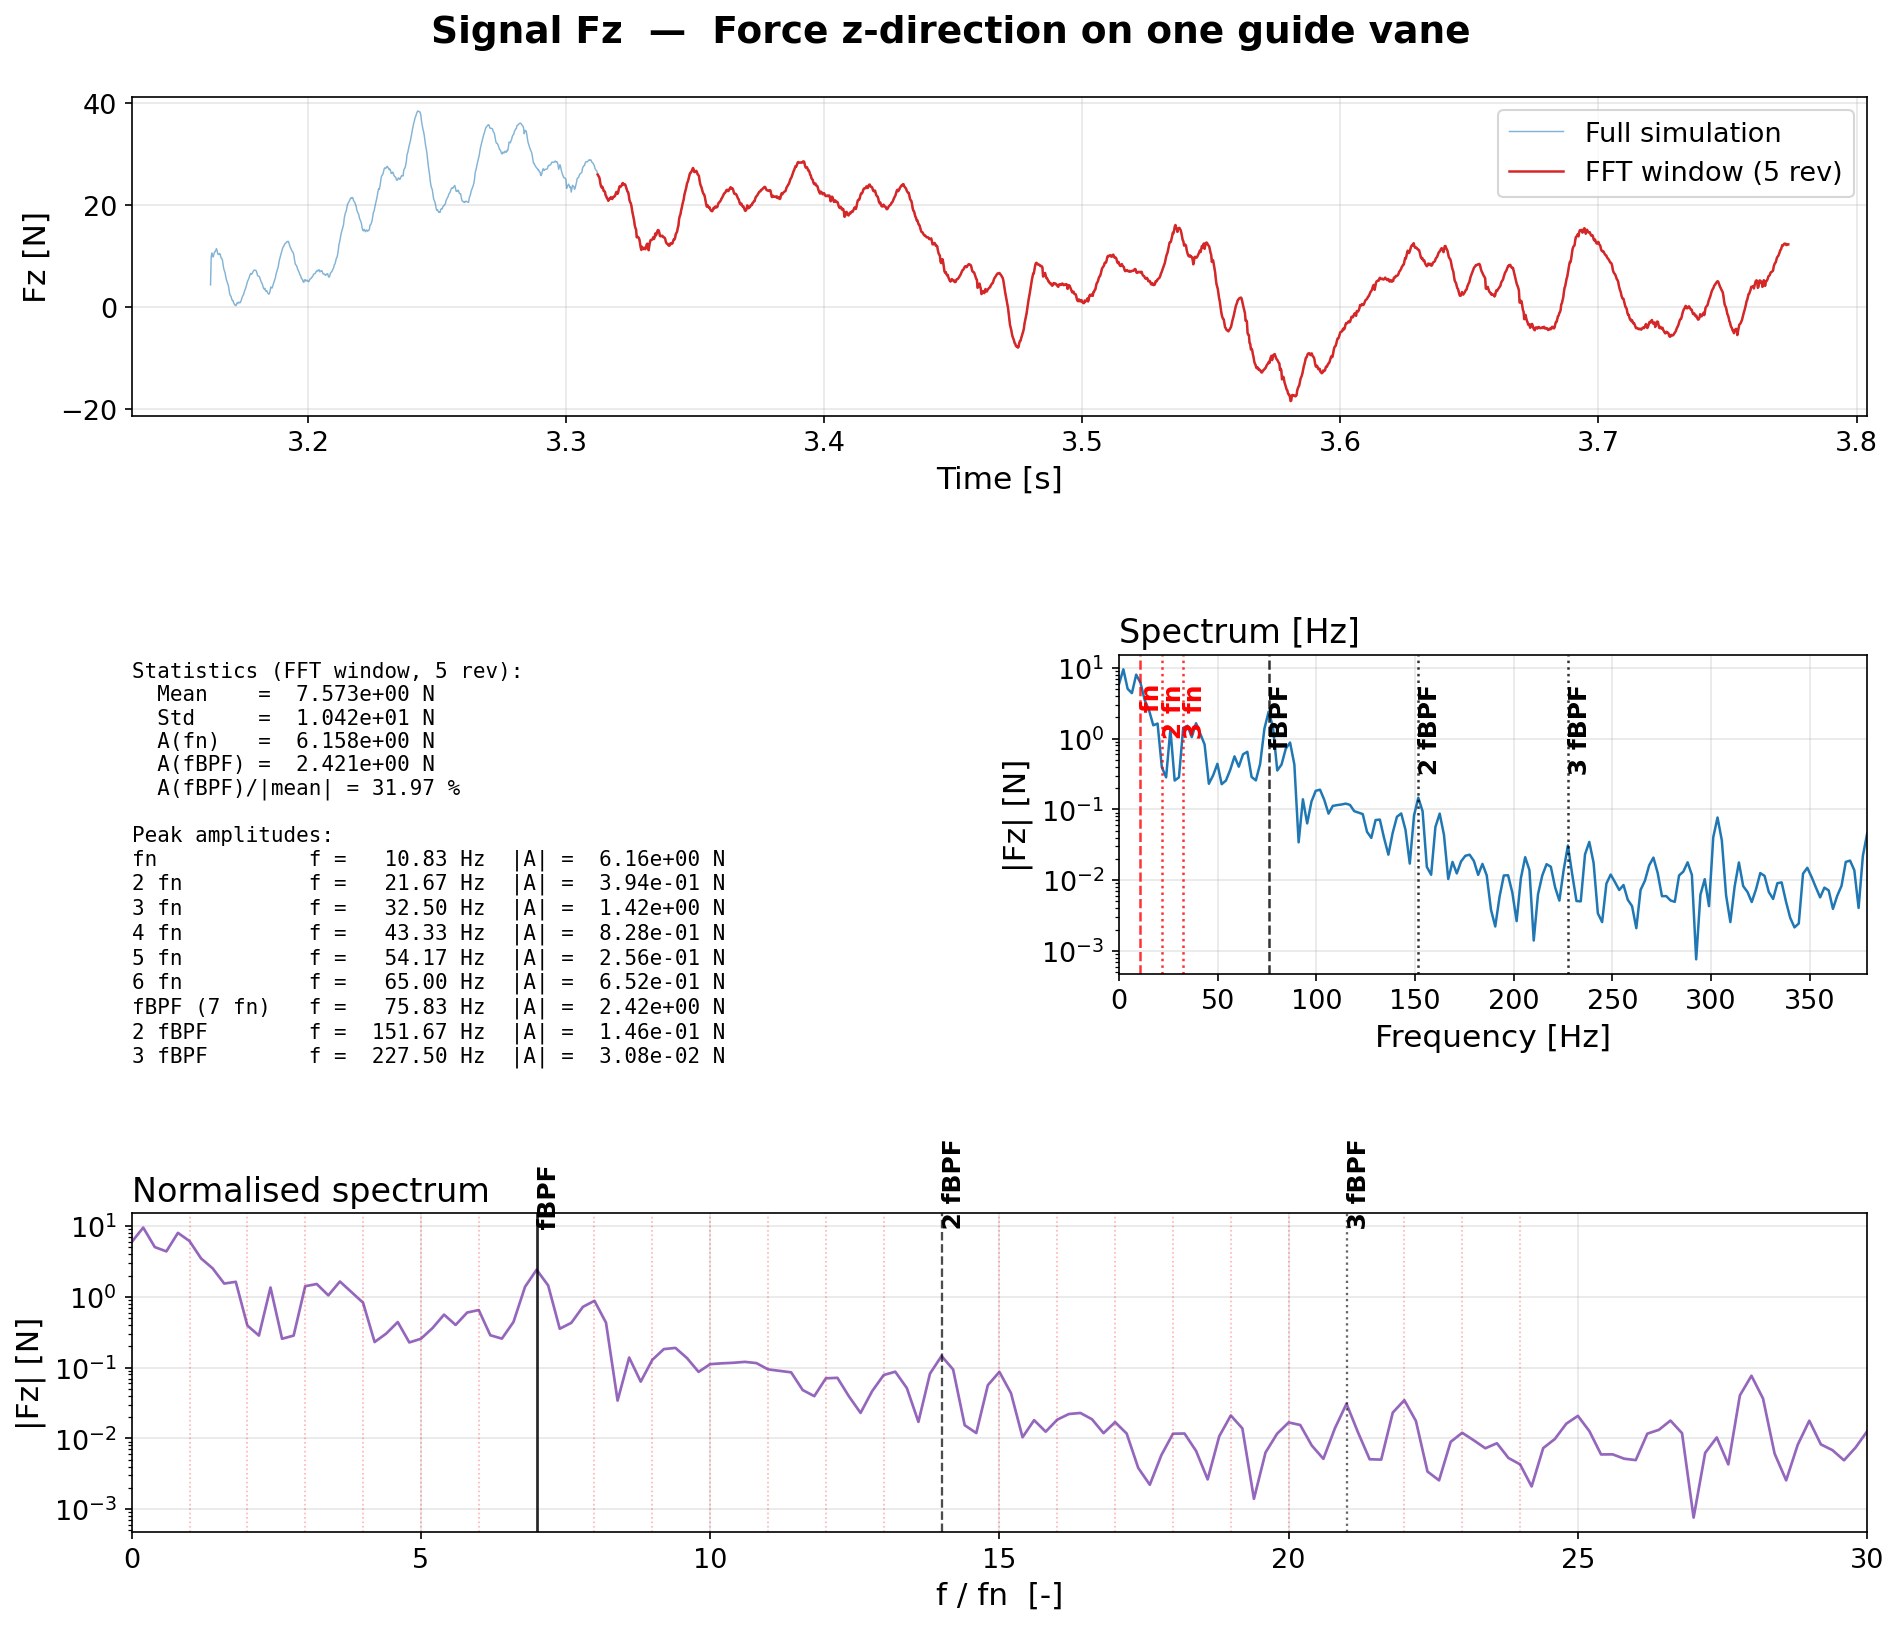
\includegraphics[width=0.95\linewidth]{Figures/FFT/signal_Fz.png}
\caption{$F_z$ — Force $z$-direction (axial) on one guide vane.}
\end{figure}

% ----- Group B: torque -------------------------------------------

\section*{Group B — Torque on the RDT}

\begin{figure}[H]\centering
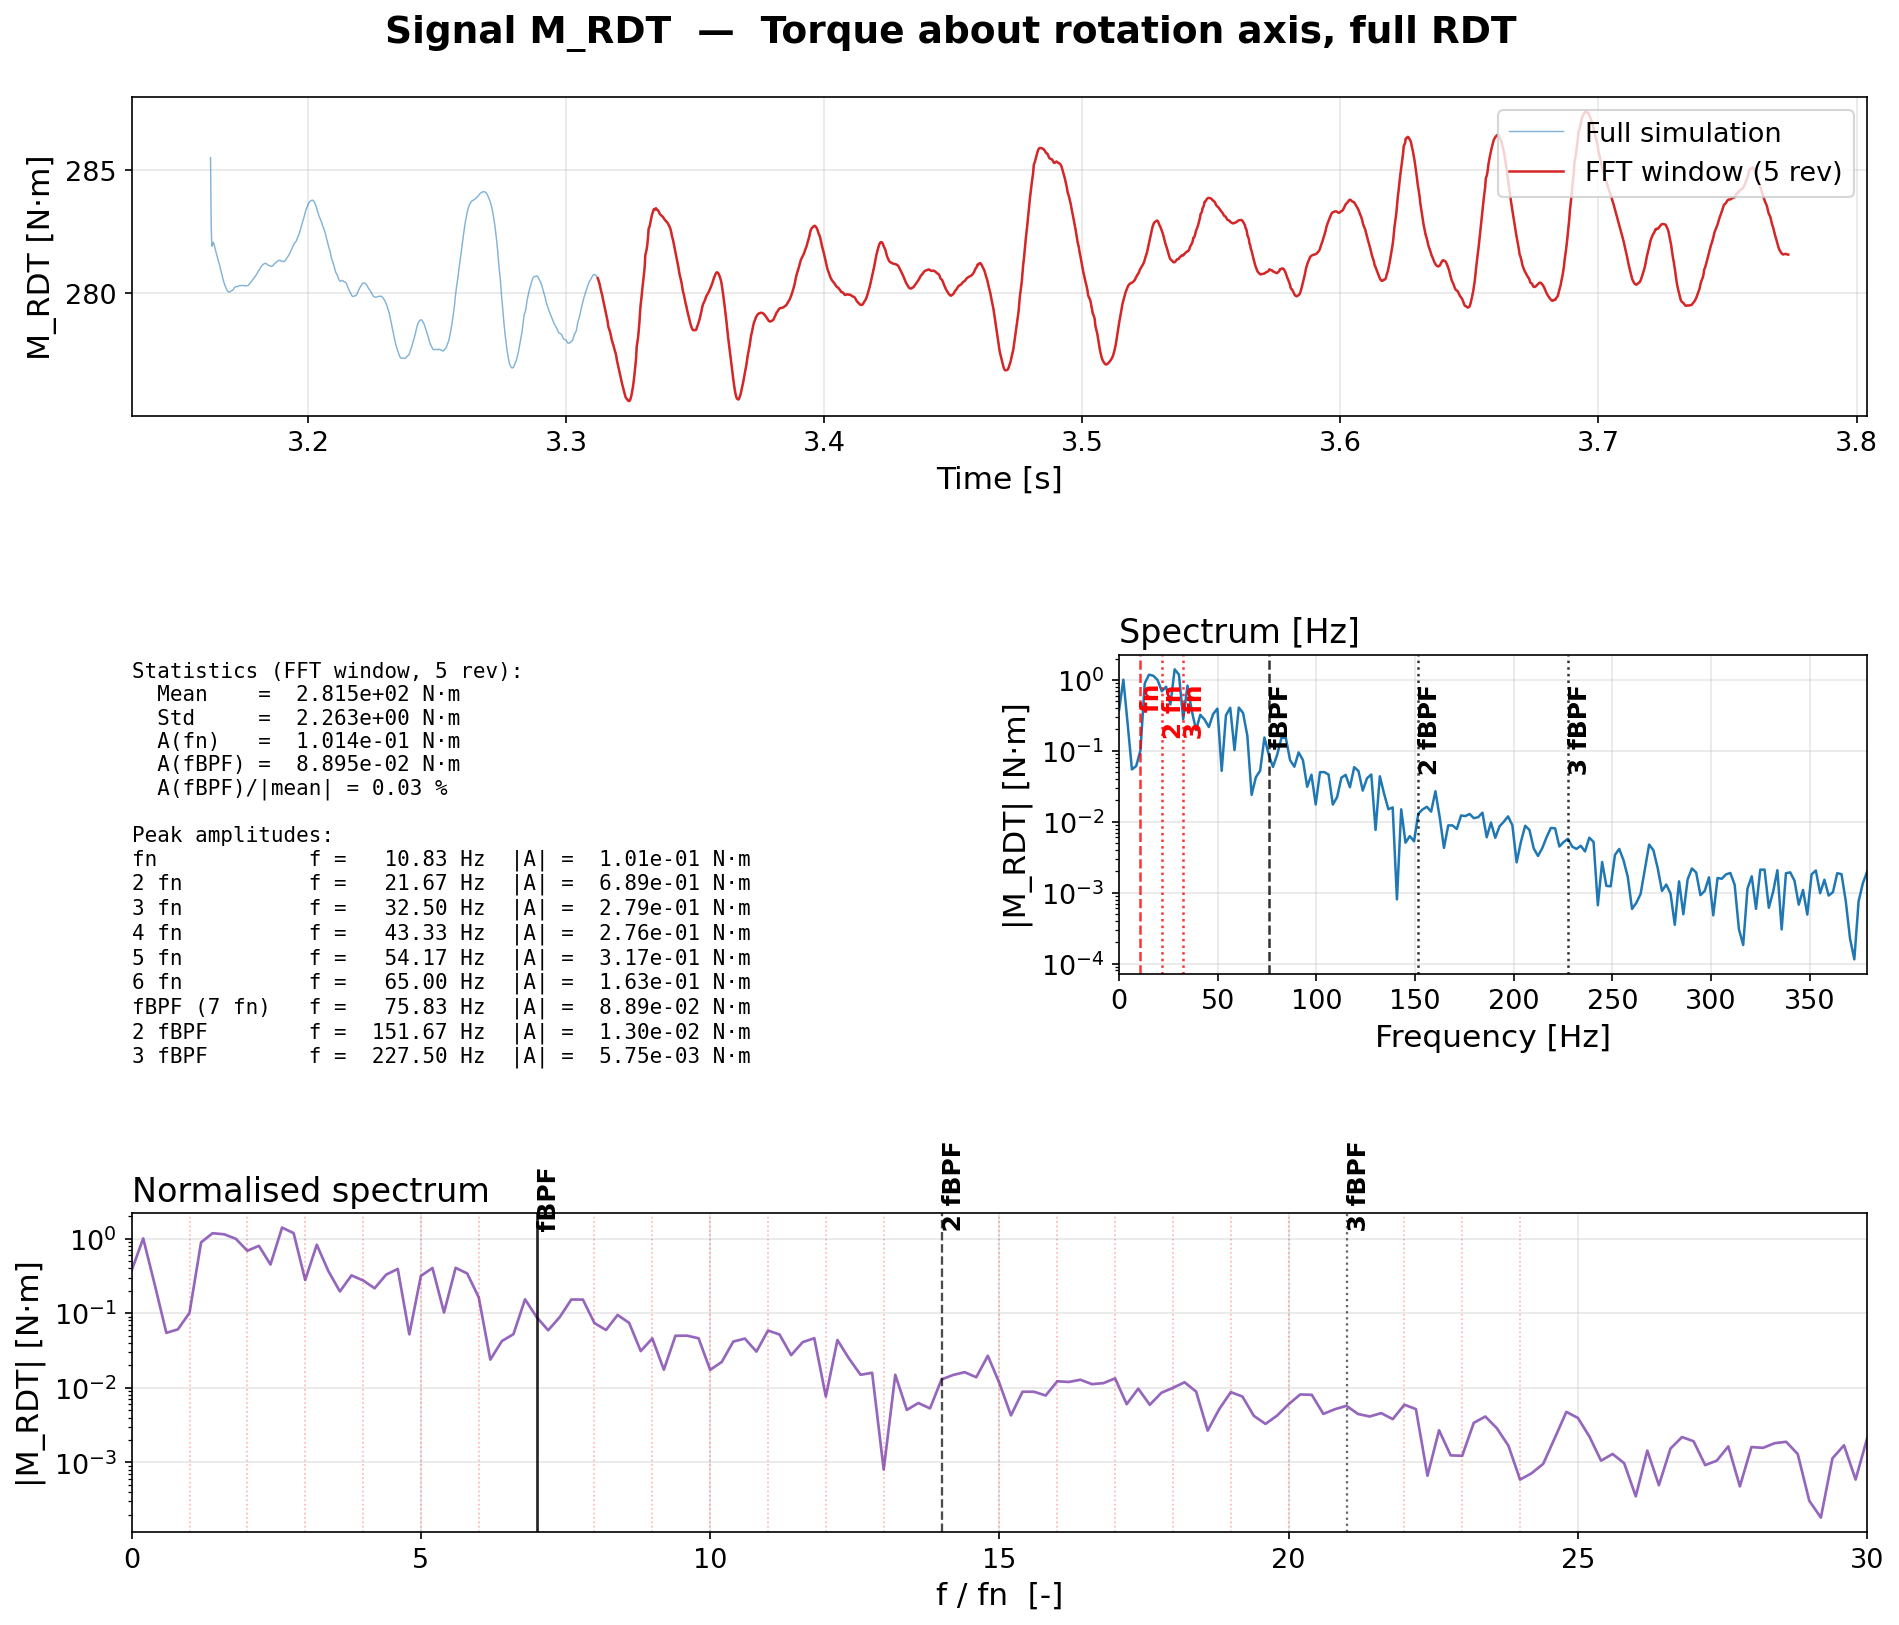
\includegraphics[width=0.95\linewidth]{Figures/FFT/signal_M_RDT.png}
\caption{$M_{\mathrm{RDT}}$ — Torque about the rotation axis,
integrated over the entire RDT blade surface.}
\end{figure}

% ----- Group C: plane-averaged pressures -------------------------

\section*{Group C — Plane-averaged pressures}

\begin{figure}[H]\centering
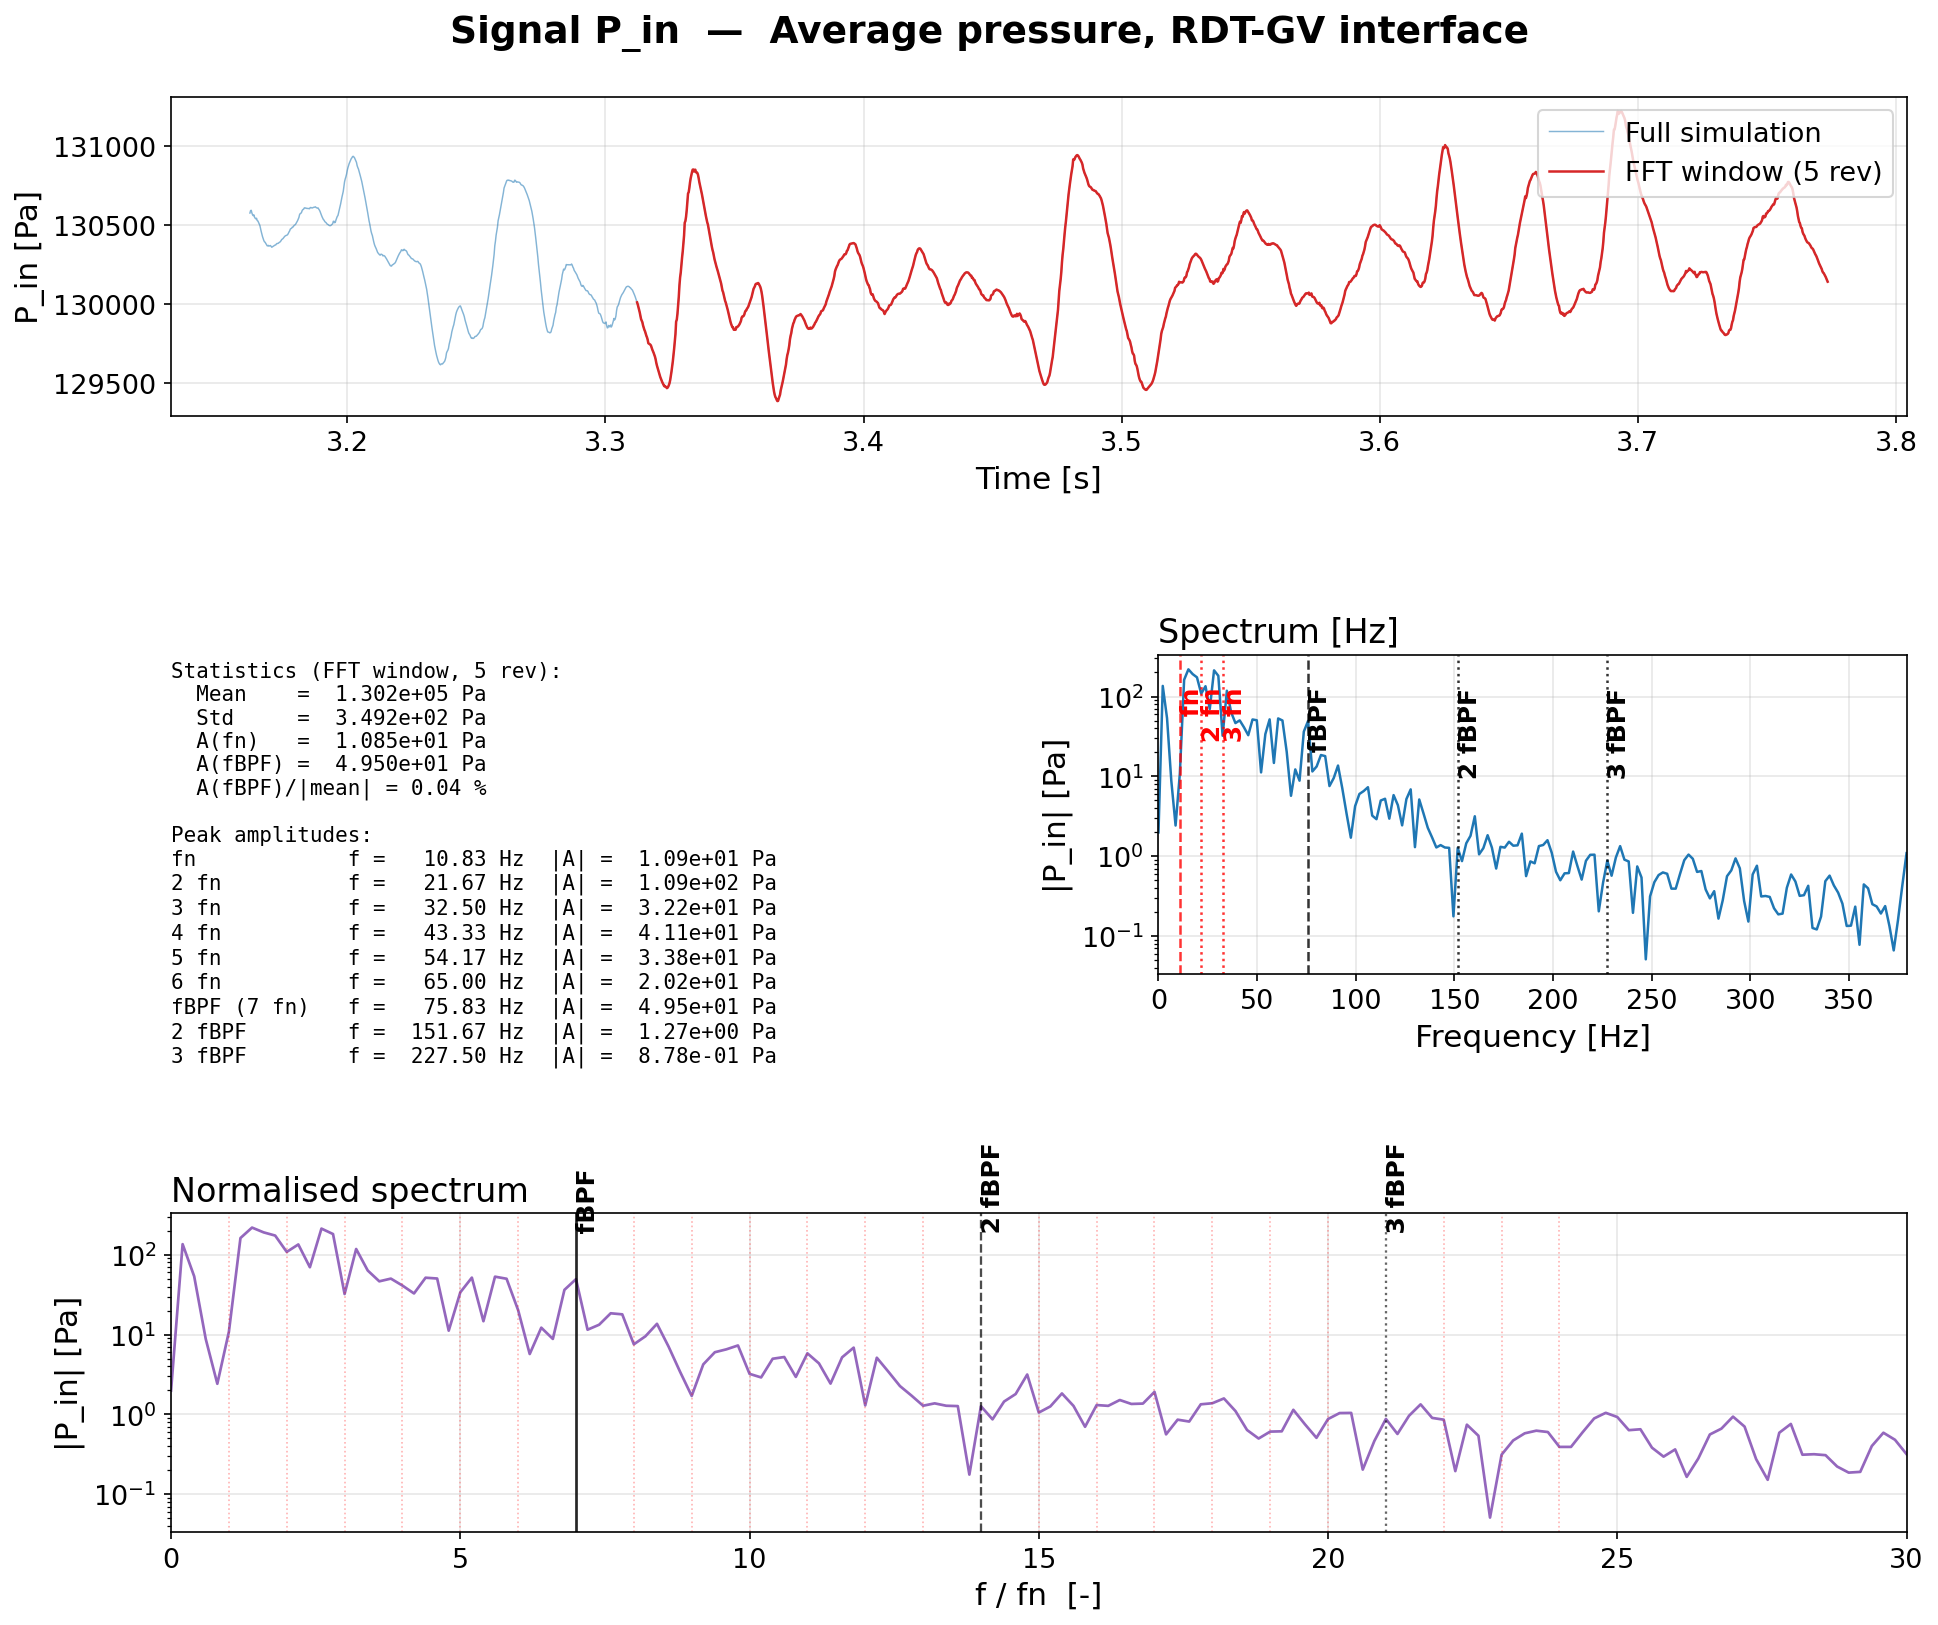
\includegraphics[width=0.95\linewidth]{Figures/FFT/signal_P_in.png}
\caption{$P_{\mathrm{in}}$ — Mass-flow-averaged pressure at the
RDT--GV interface ($s = 0$~mm).}
\end{figure}

\begin{figure}[H]\centering
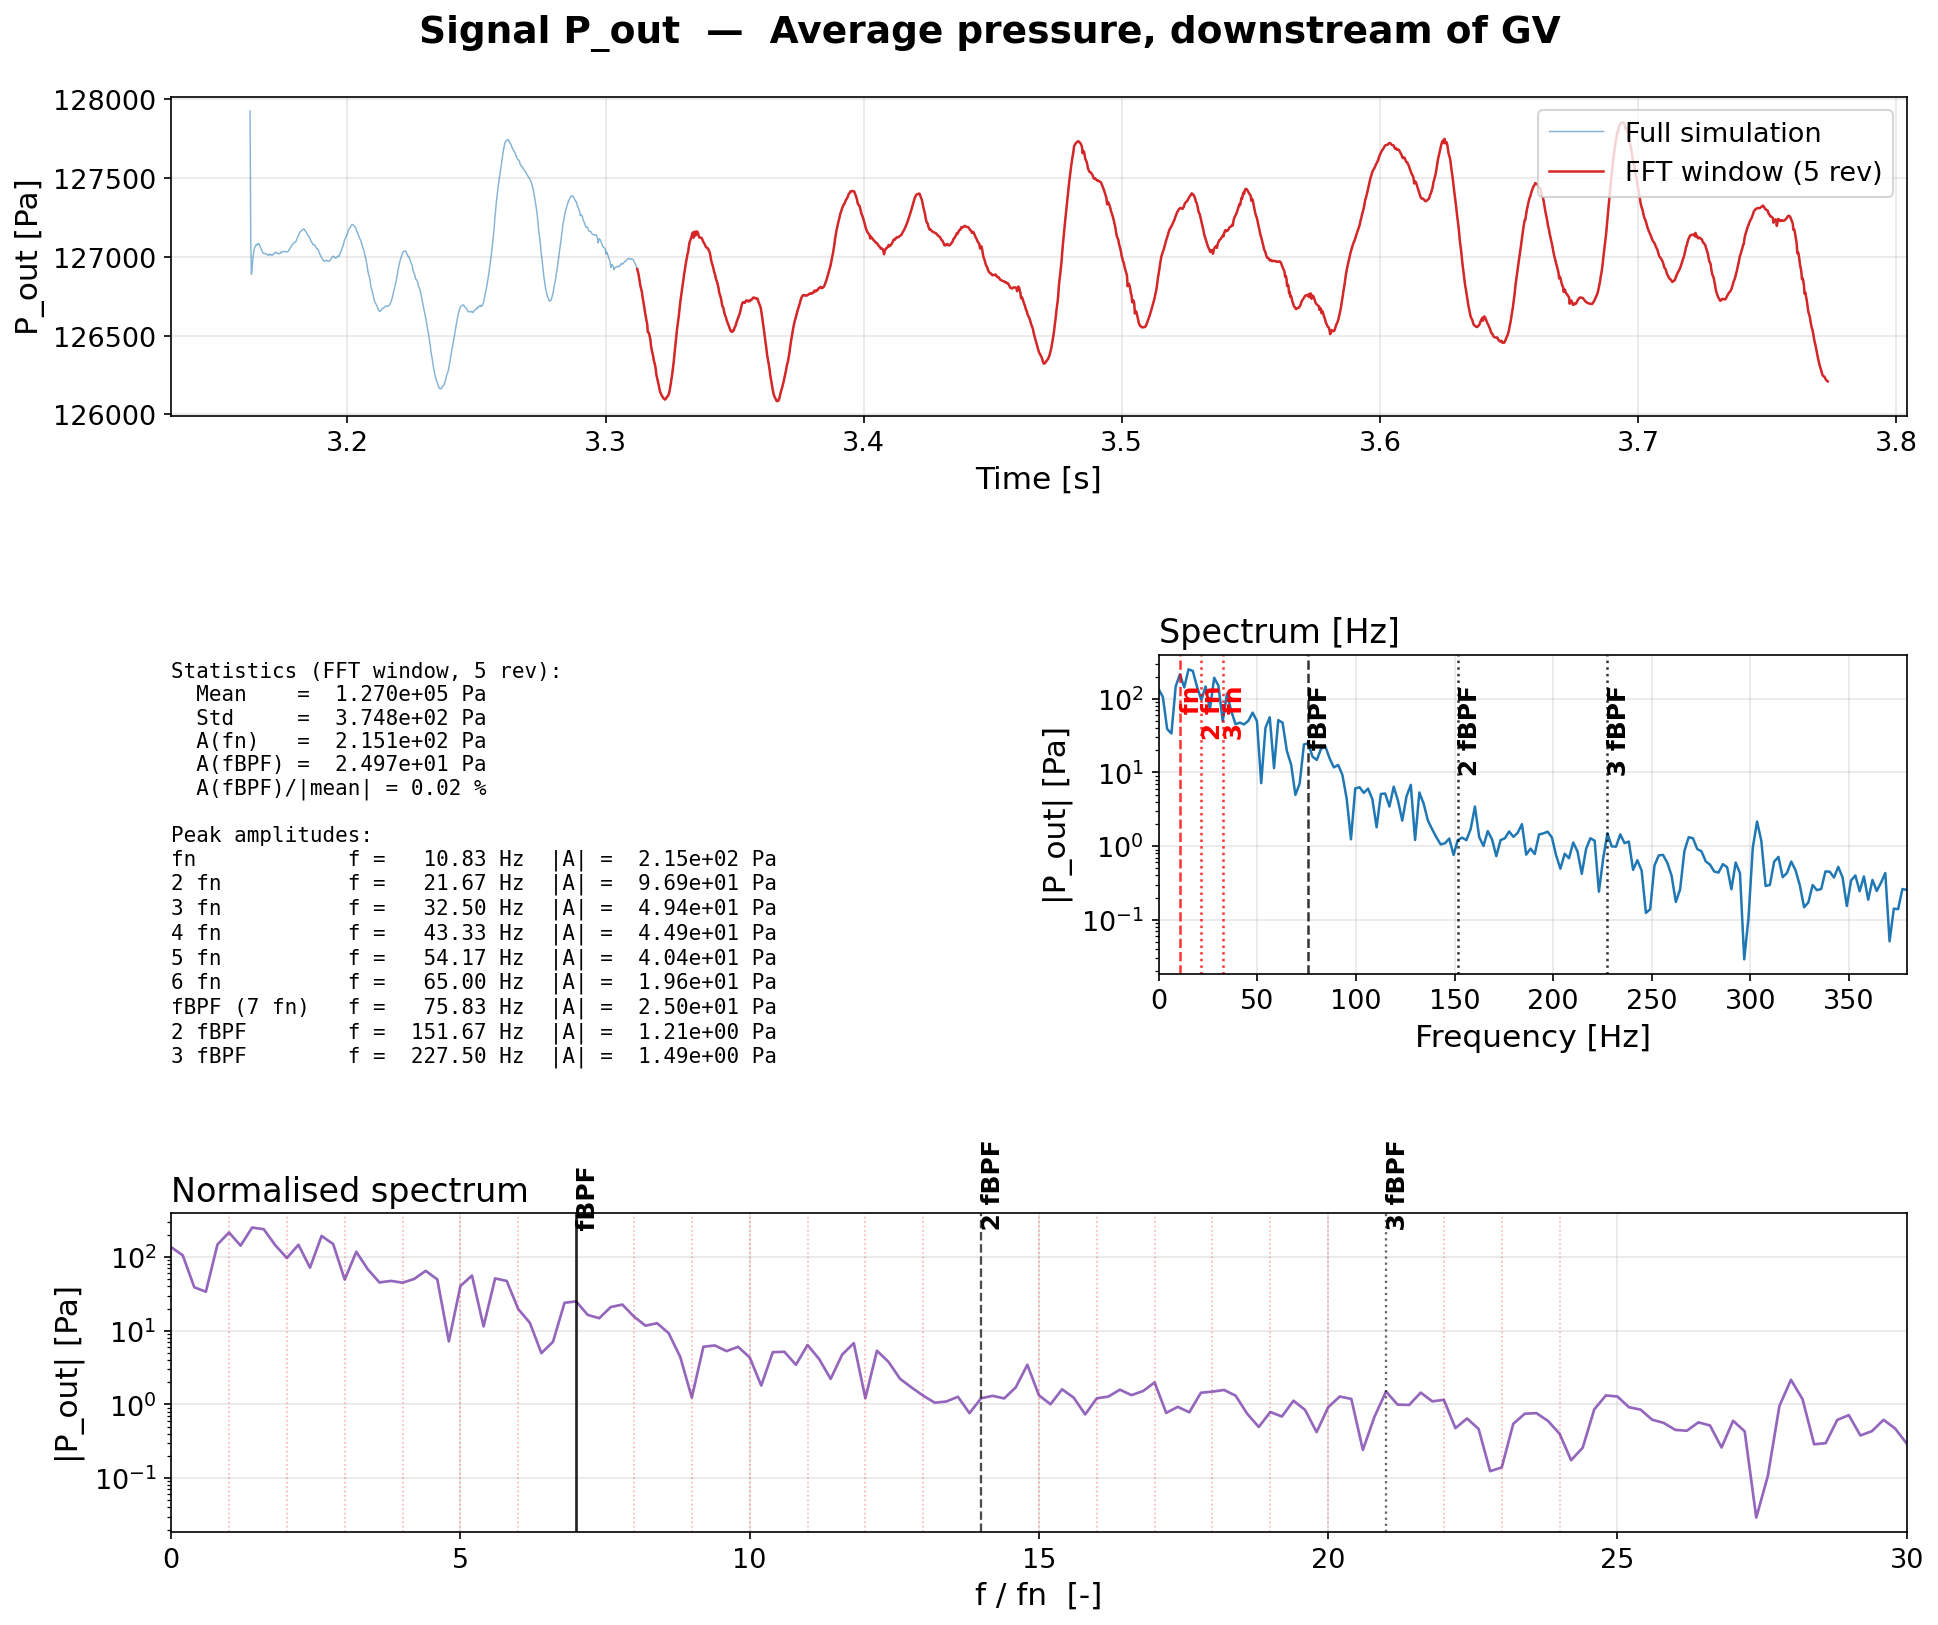
\includegraphics[width=0.95\linewidth]{Figures/FFT/signal_P_out.png}
\caption{$P_{\mathrm{out}}$ — Mass-flow-averaged pressure
downstream of the GV row ($s = 500$~mm).}
\end{figure}

\begin{figure}[H]\centering
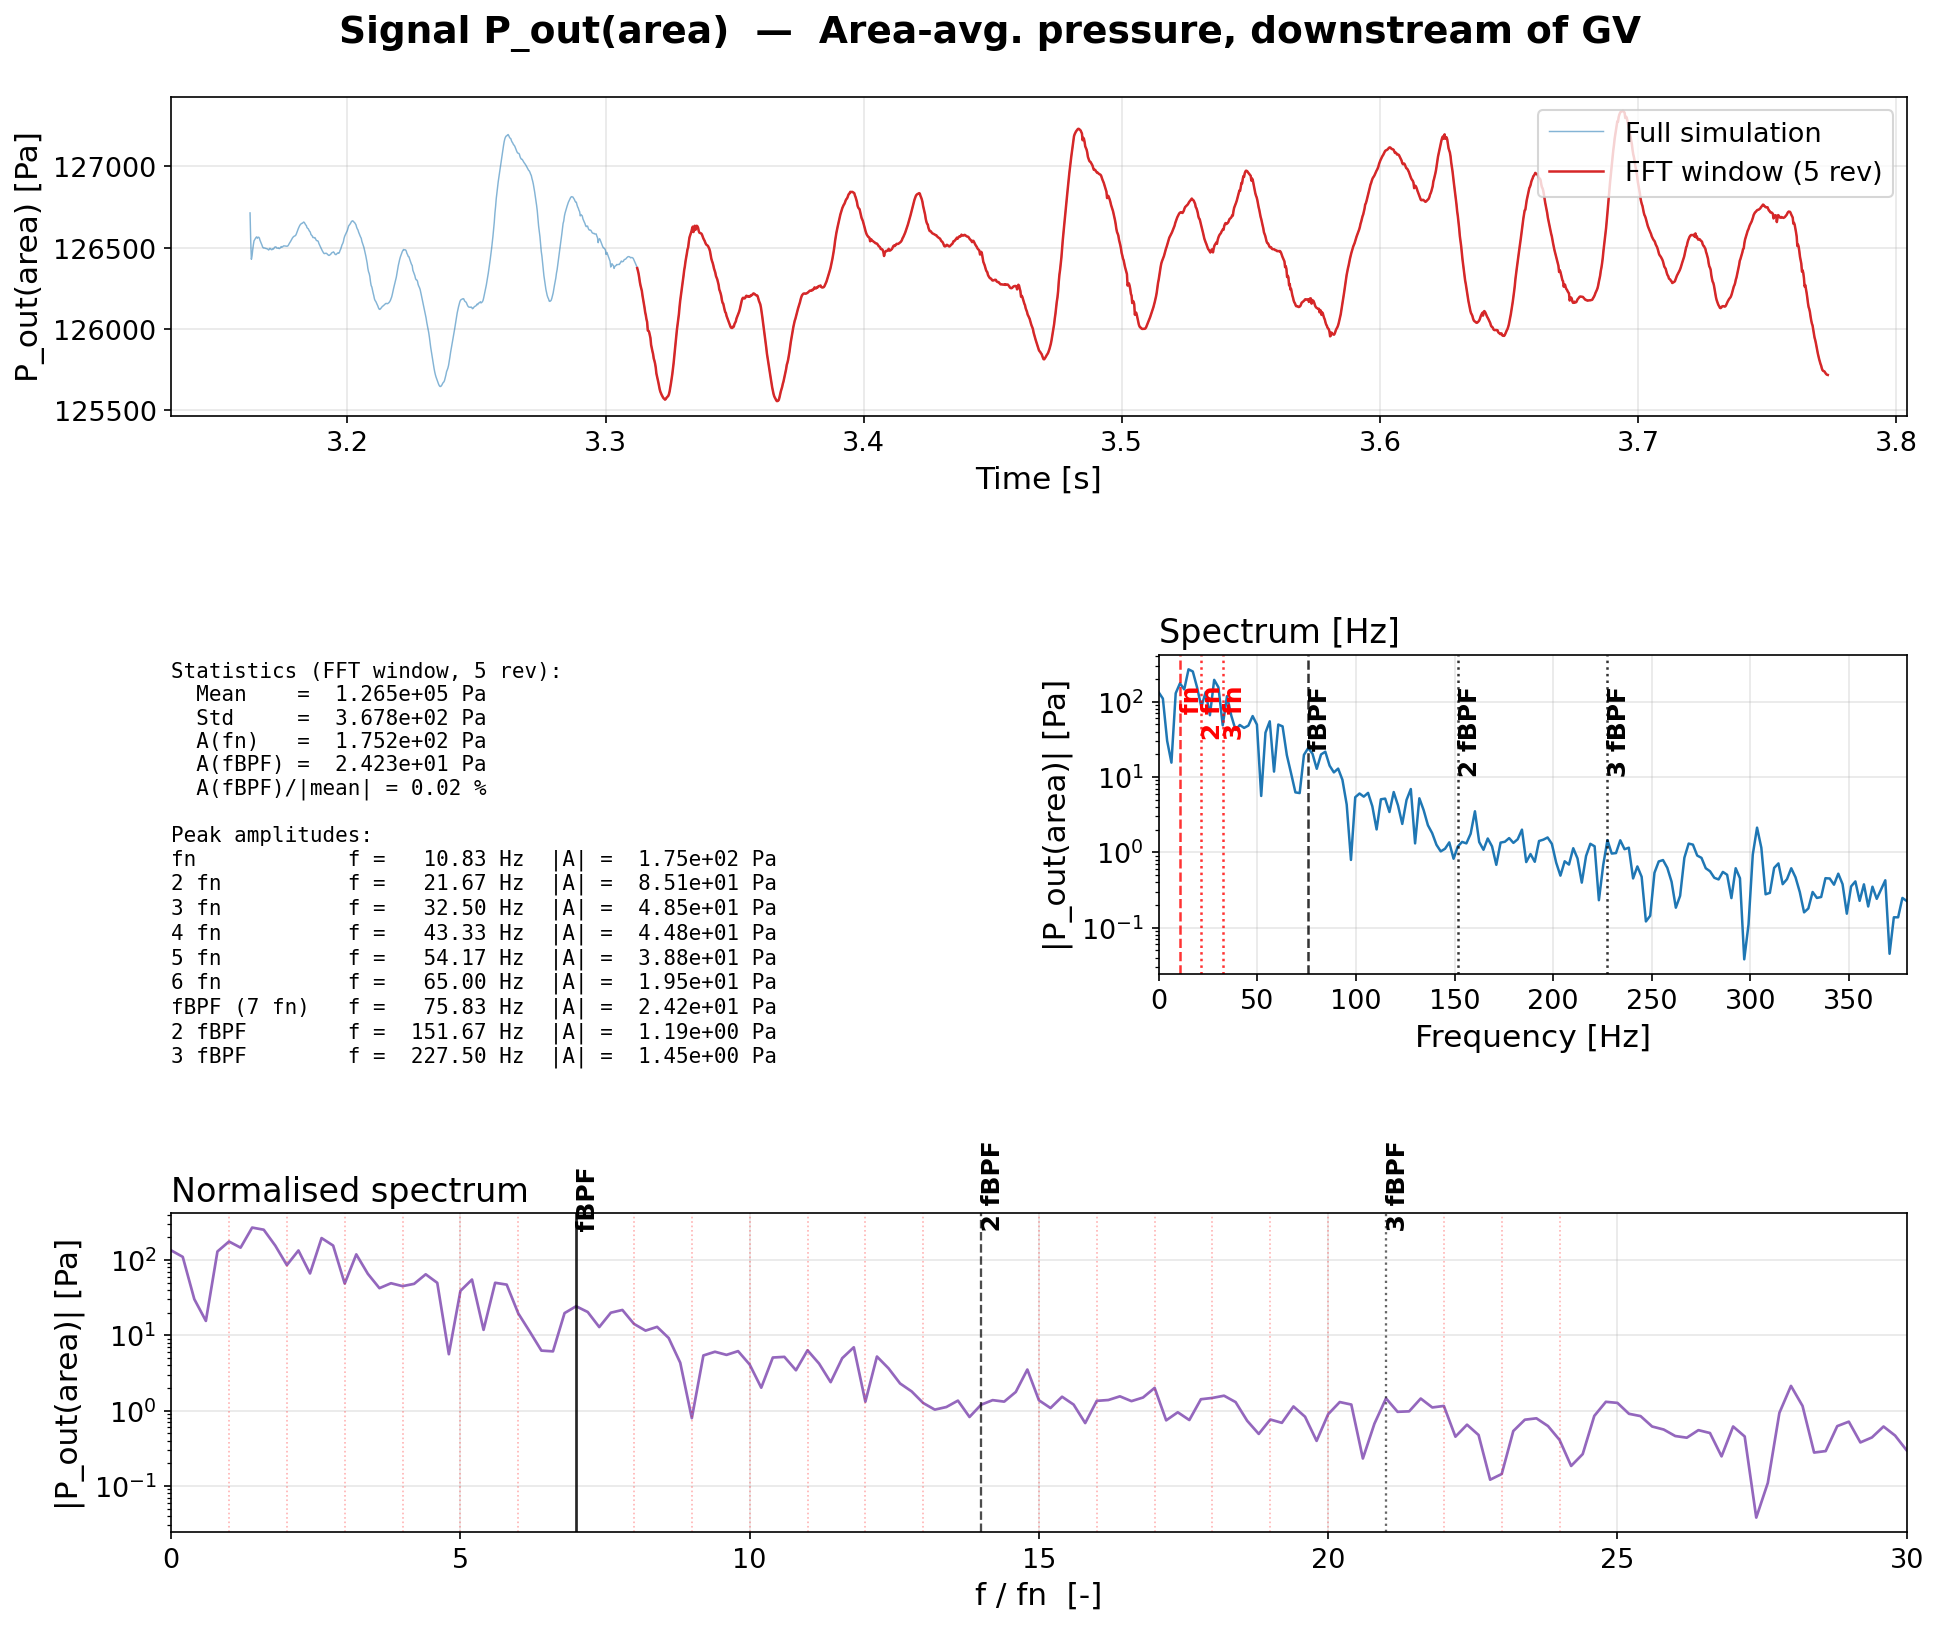
\includegraphics[width=0.95\linewidth]{Figures/FFT/signal_P_out_area.png}
\caption{$P_{\mathrm{out}}^{\,a}$ — Area-averaged pressure
downstream of the GV row (reference check only).}
\end{figure}

% ----- Group D: centre-of-pipe before bend -----------------------

\section*{Group D — Centre of pipe before the 90$^\circ$ bend}

\begin{figure}[H]\centering
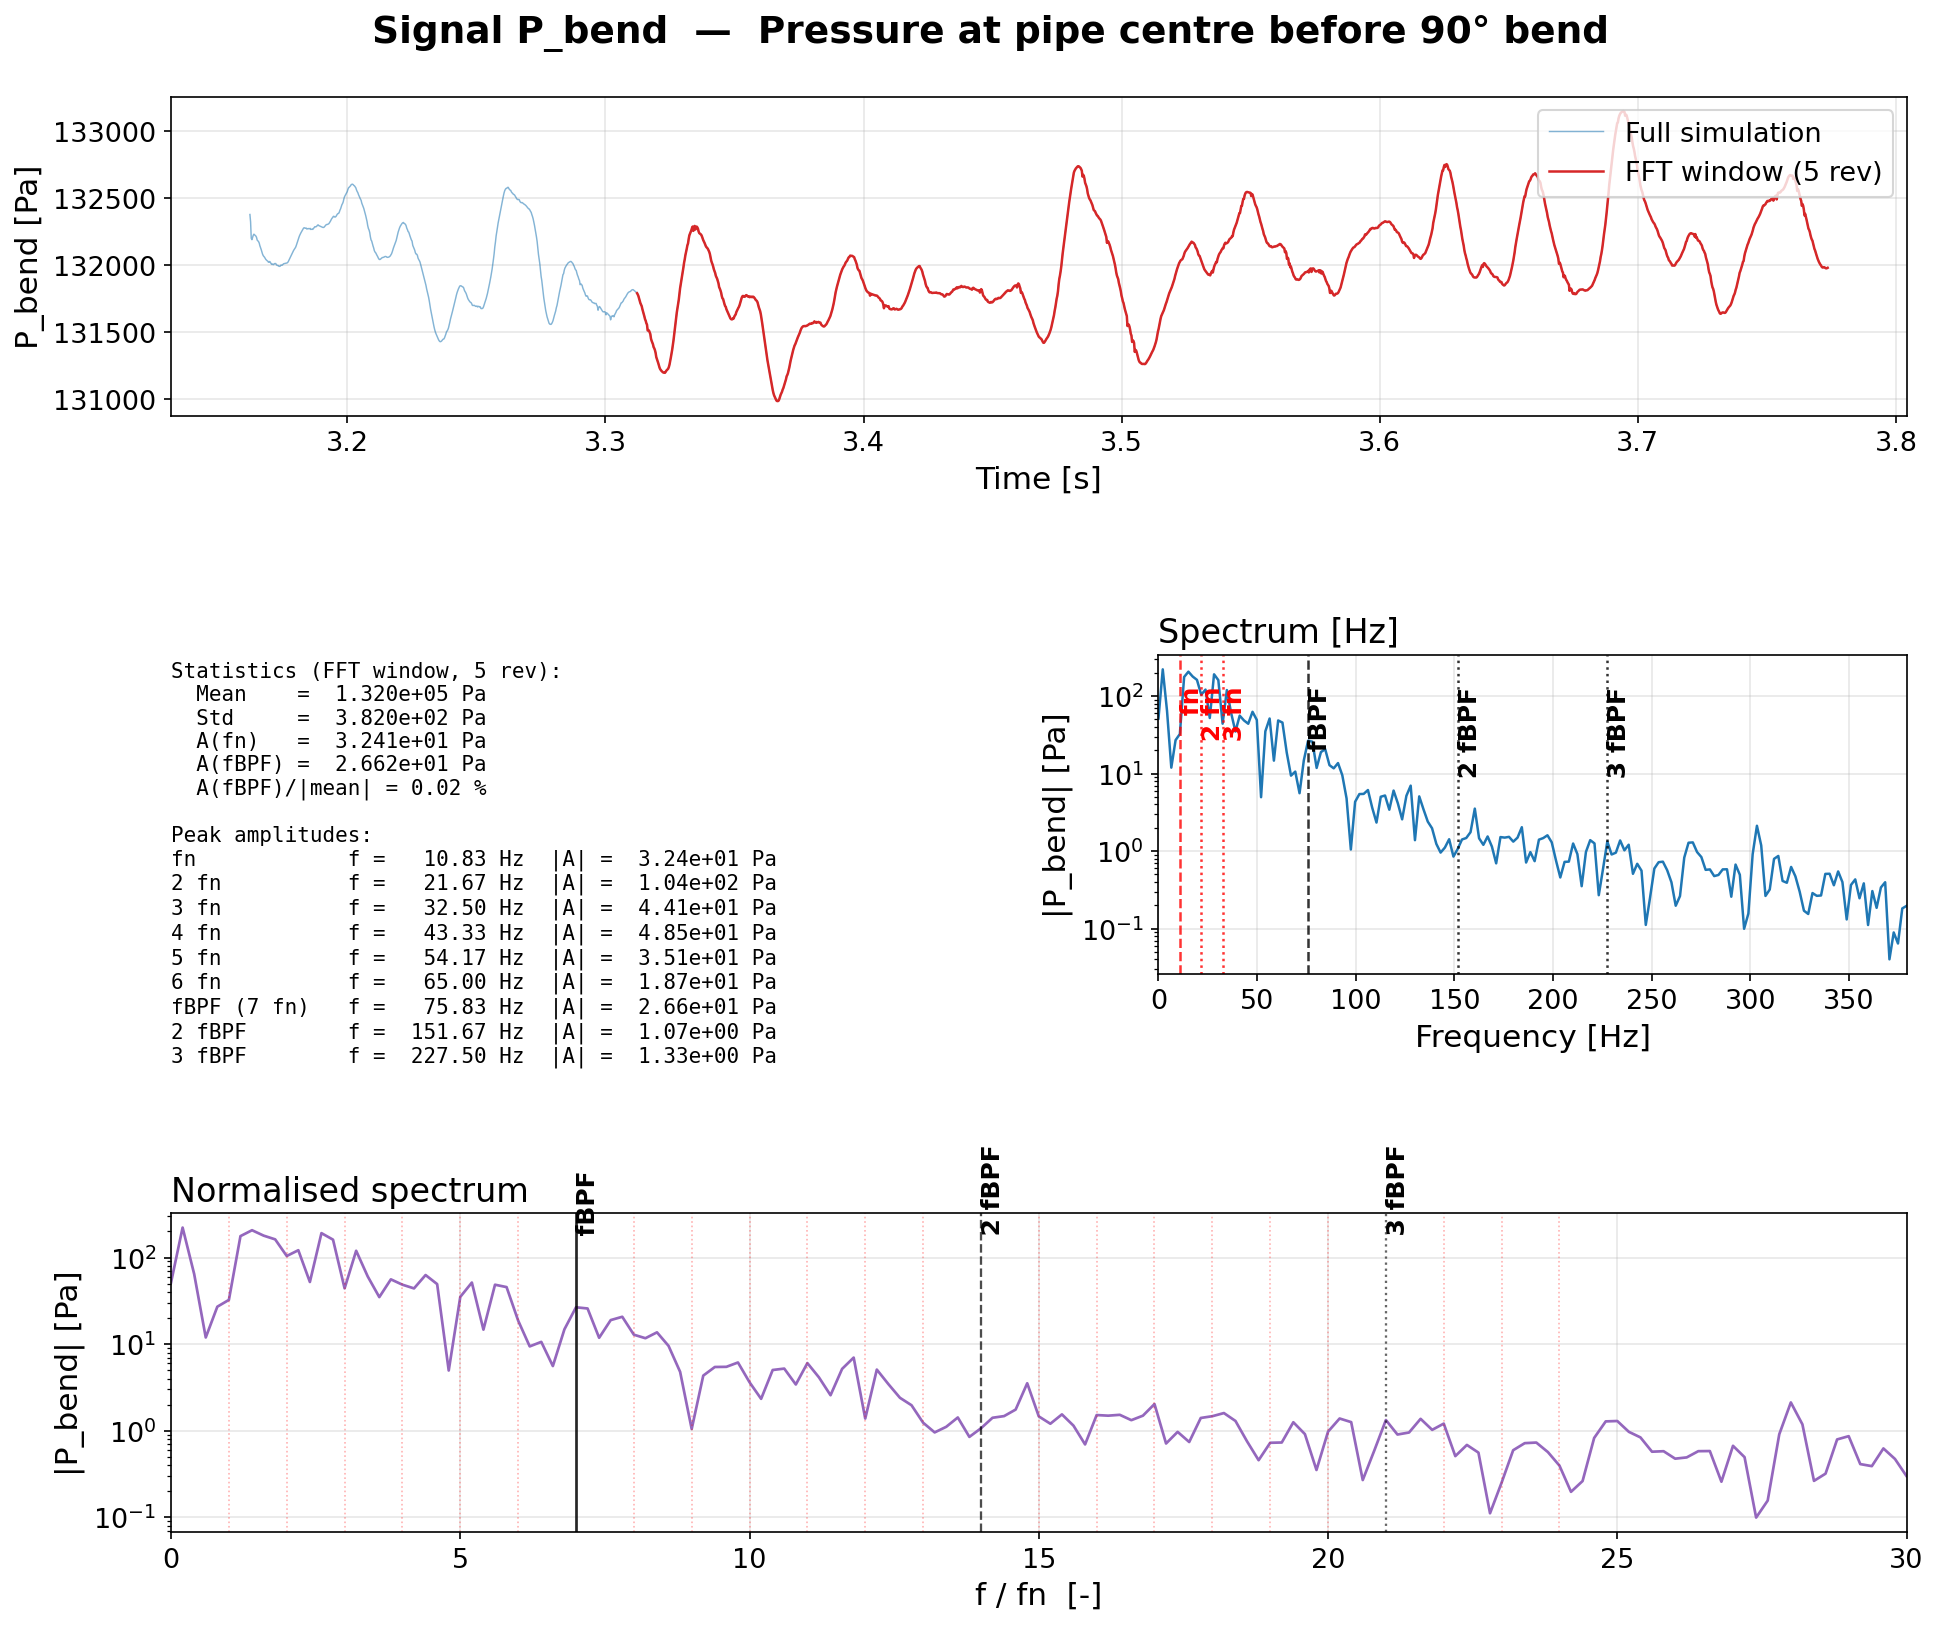
\includegraphics[width=0.95\linewidth]{Figures/FFT/signal_P_bend.png}
\caption{$P_{\mathrm{bend}}$ — Pressure at the centre of the pipe
before the 90$^\circ$ bend ($z = -2.185$~m).}
\end{figure}

% ----- Group E: wall probes along the GV passage -----------------

\section*{Group E — Wall-pressure probes along the GV passage}

\begin{figure}[H]\centering
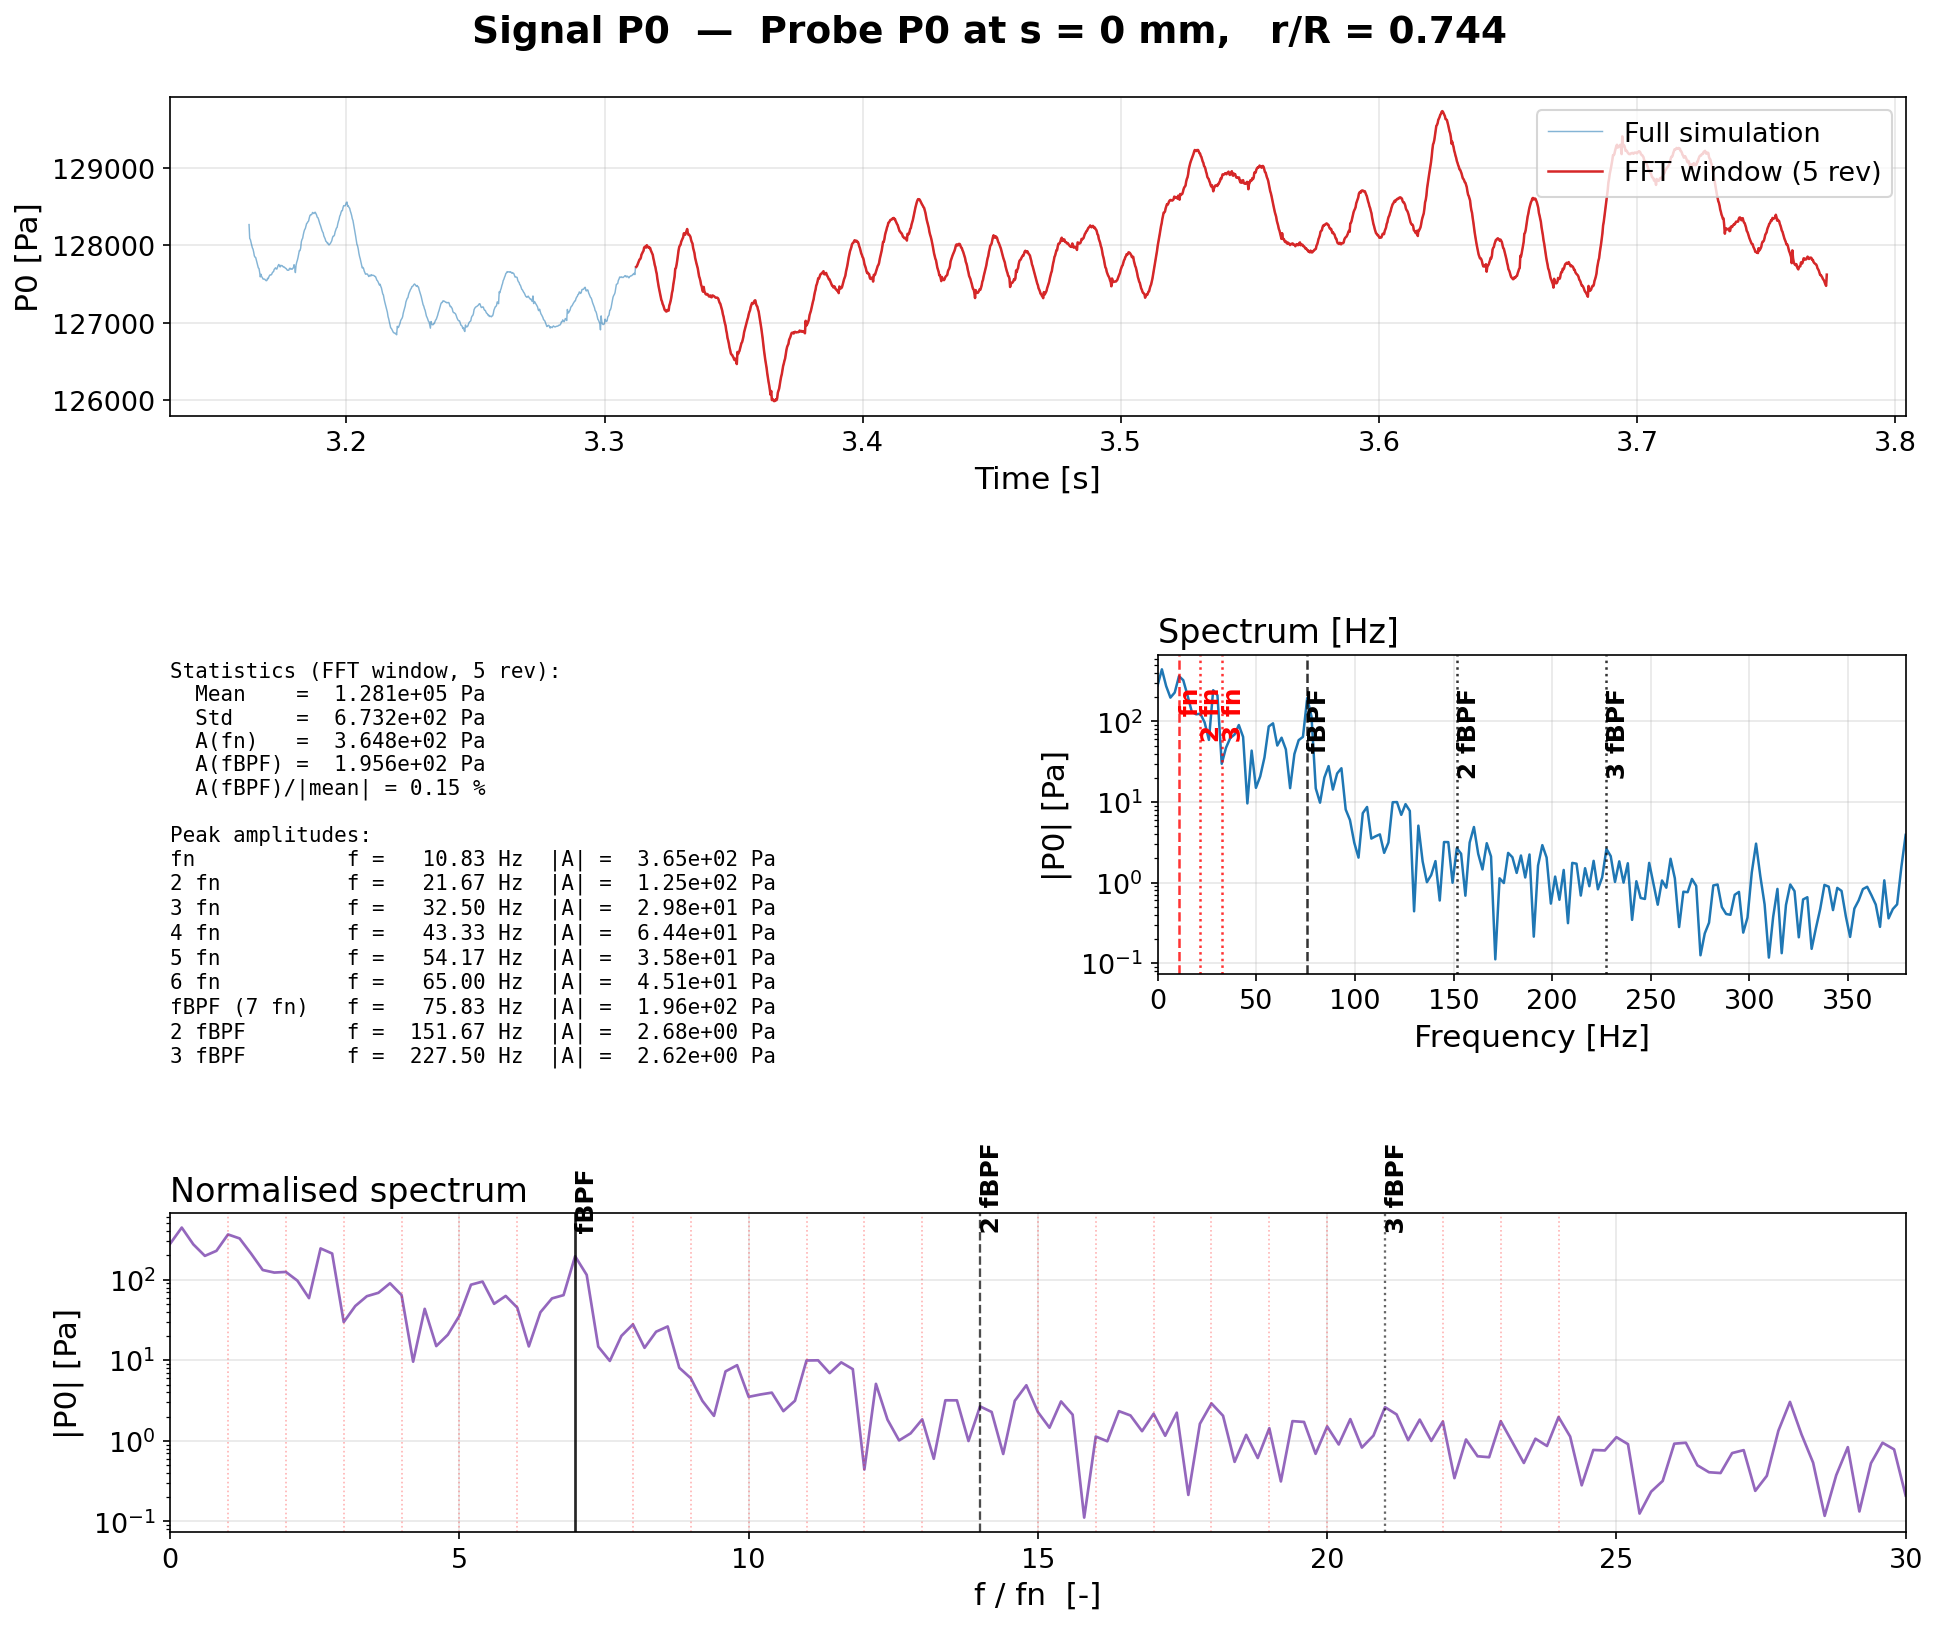
\includegraphics[width=0.95\linewidth]{Figures/FFT/signal_P0.png}
\caption{$P_0$ — Wall probe at $s = 0$~mm, $r/R = 0.744$.}
\end{figure}

\begin{figure}[H]\centering
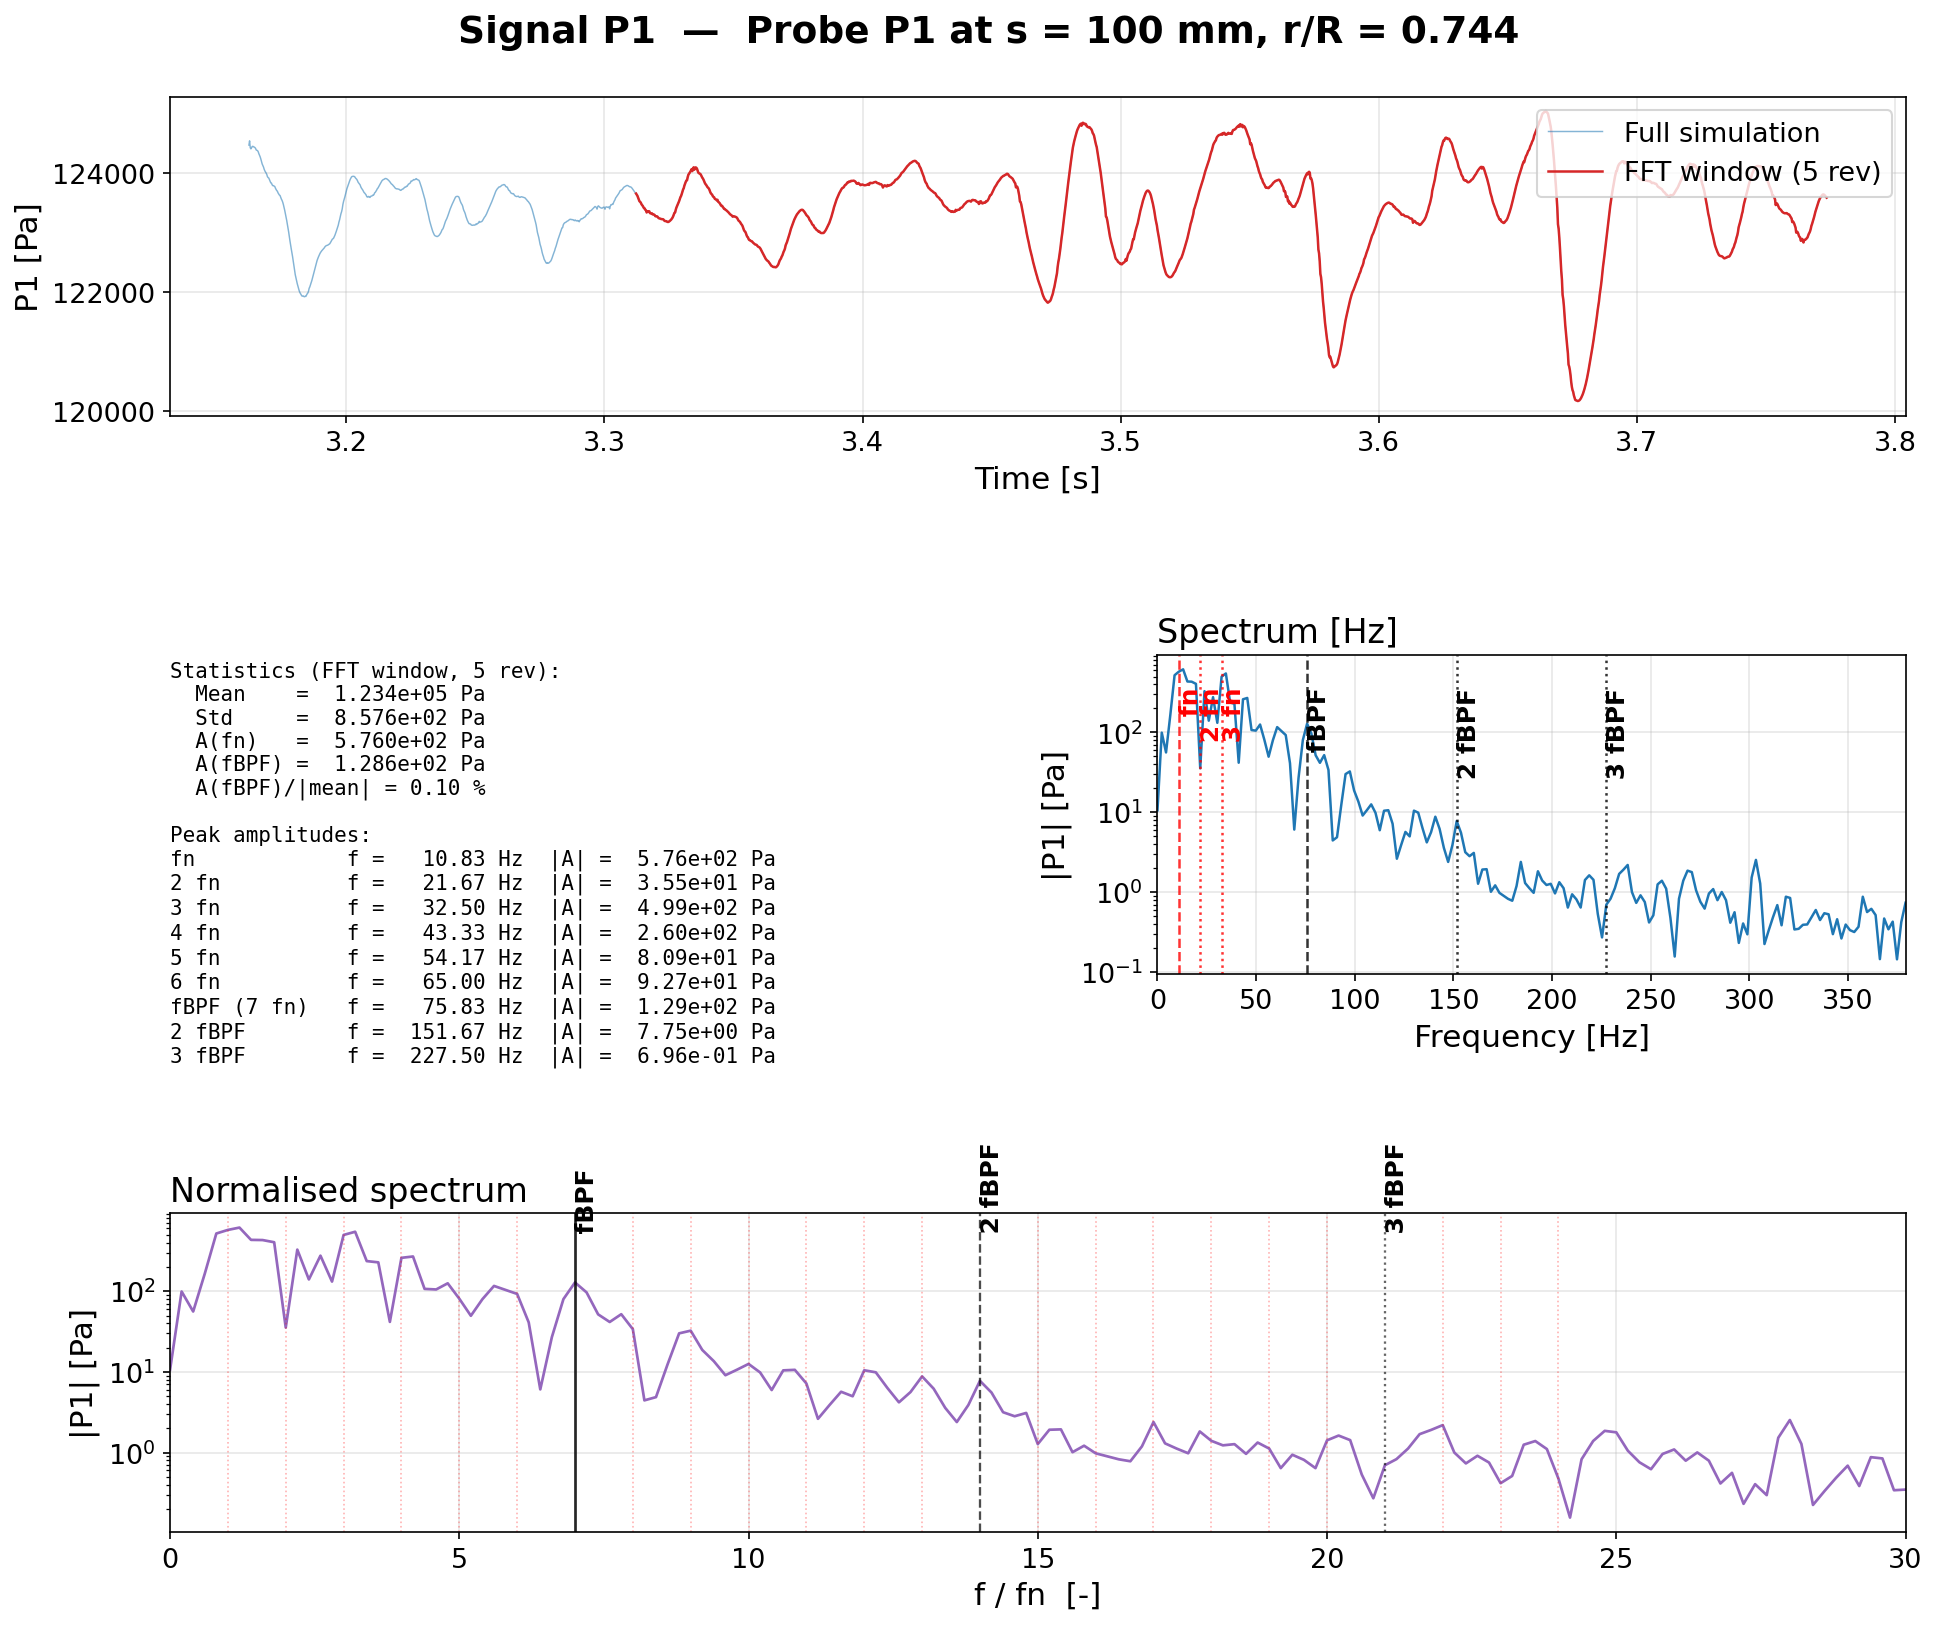
\includegraphics[width=0.95\linewidth]{Figures/FFT/signal_P1.png}
\caption{$P_1$ — Wall probe at $s = 100$~mm, $r/R = 0.744$.}
\end{figure}

\begin{figure}[H]\centering
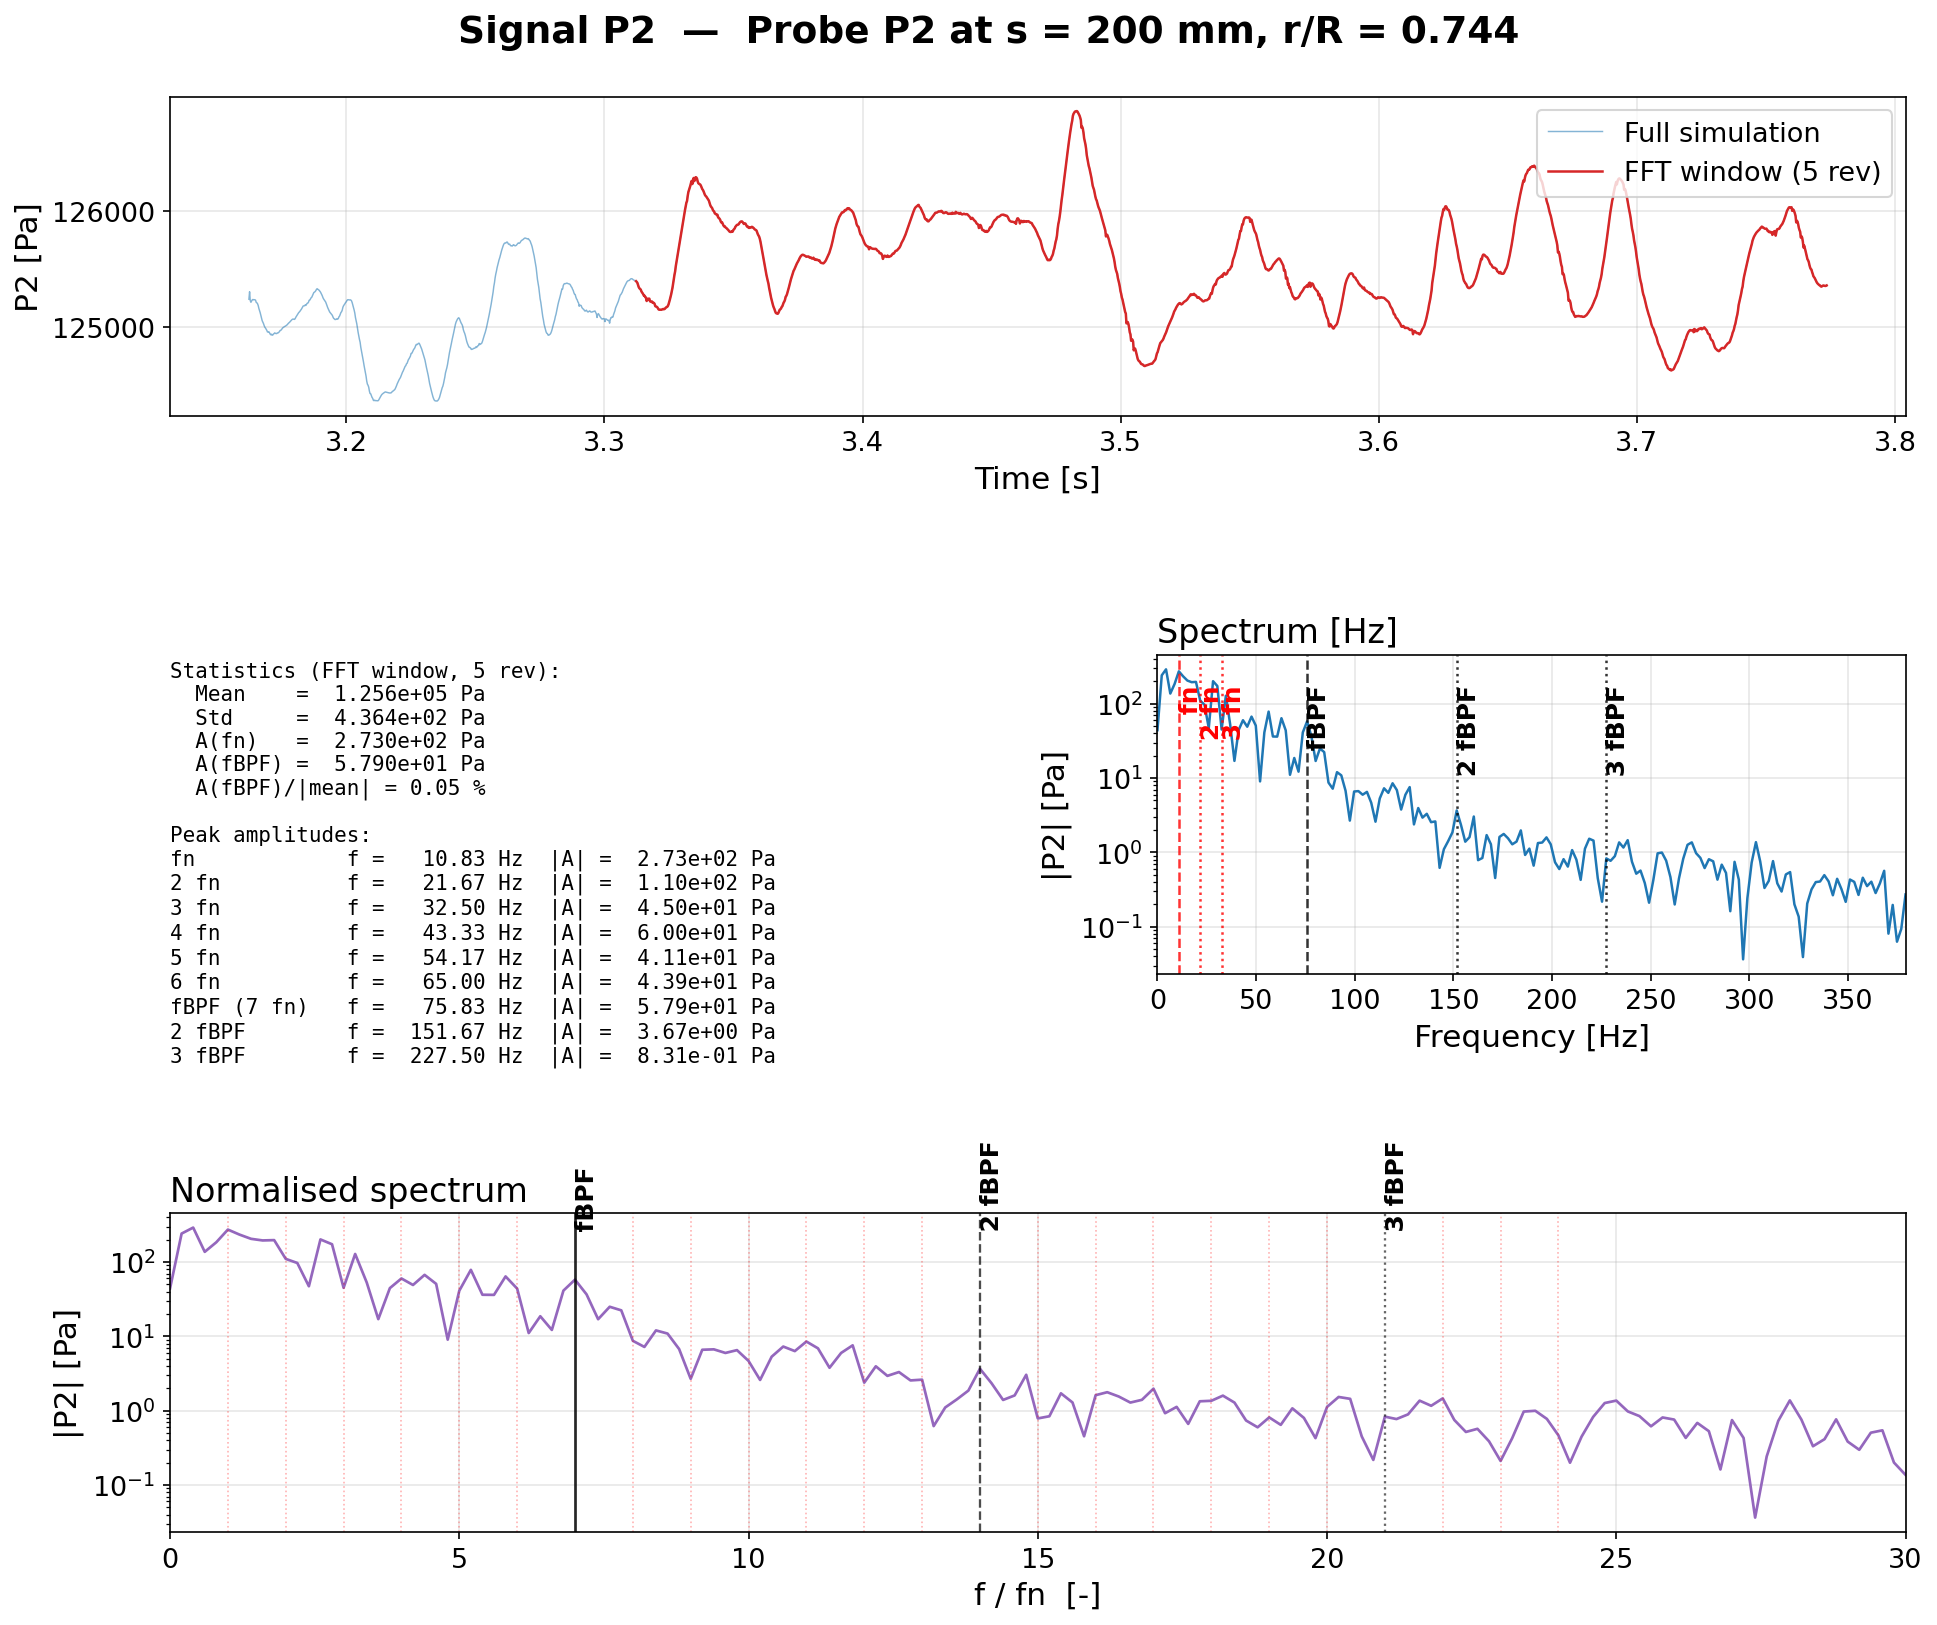
\includegraphics[width=0.95\linewidth]{Figures/FFT/signal_P2.png}
\caption{$P_2$ — Wall probe at $s = 200$~mm, $r/R = 0.744$.}
\end{figure}

\begin{figure}[H]\centering
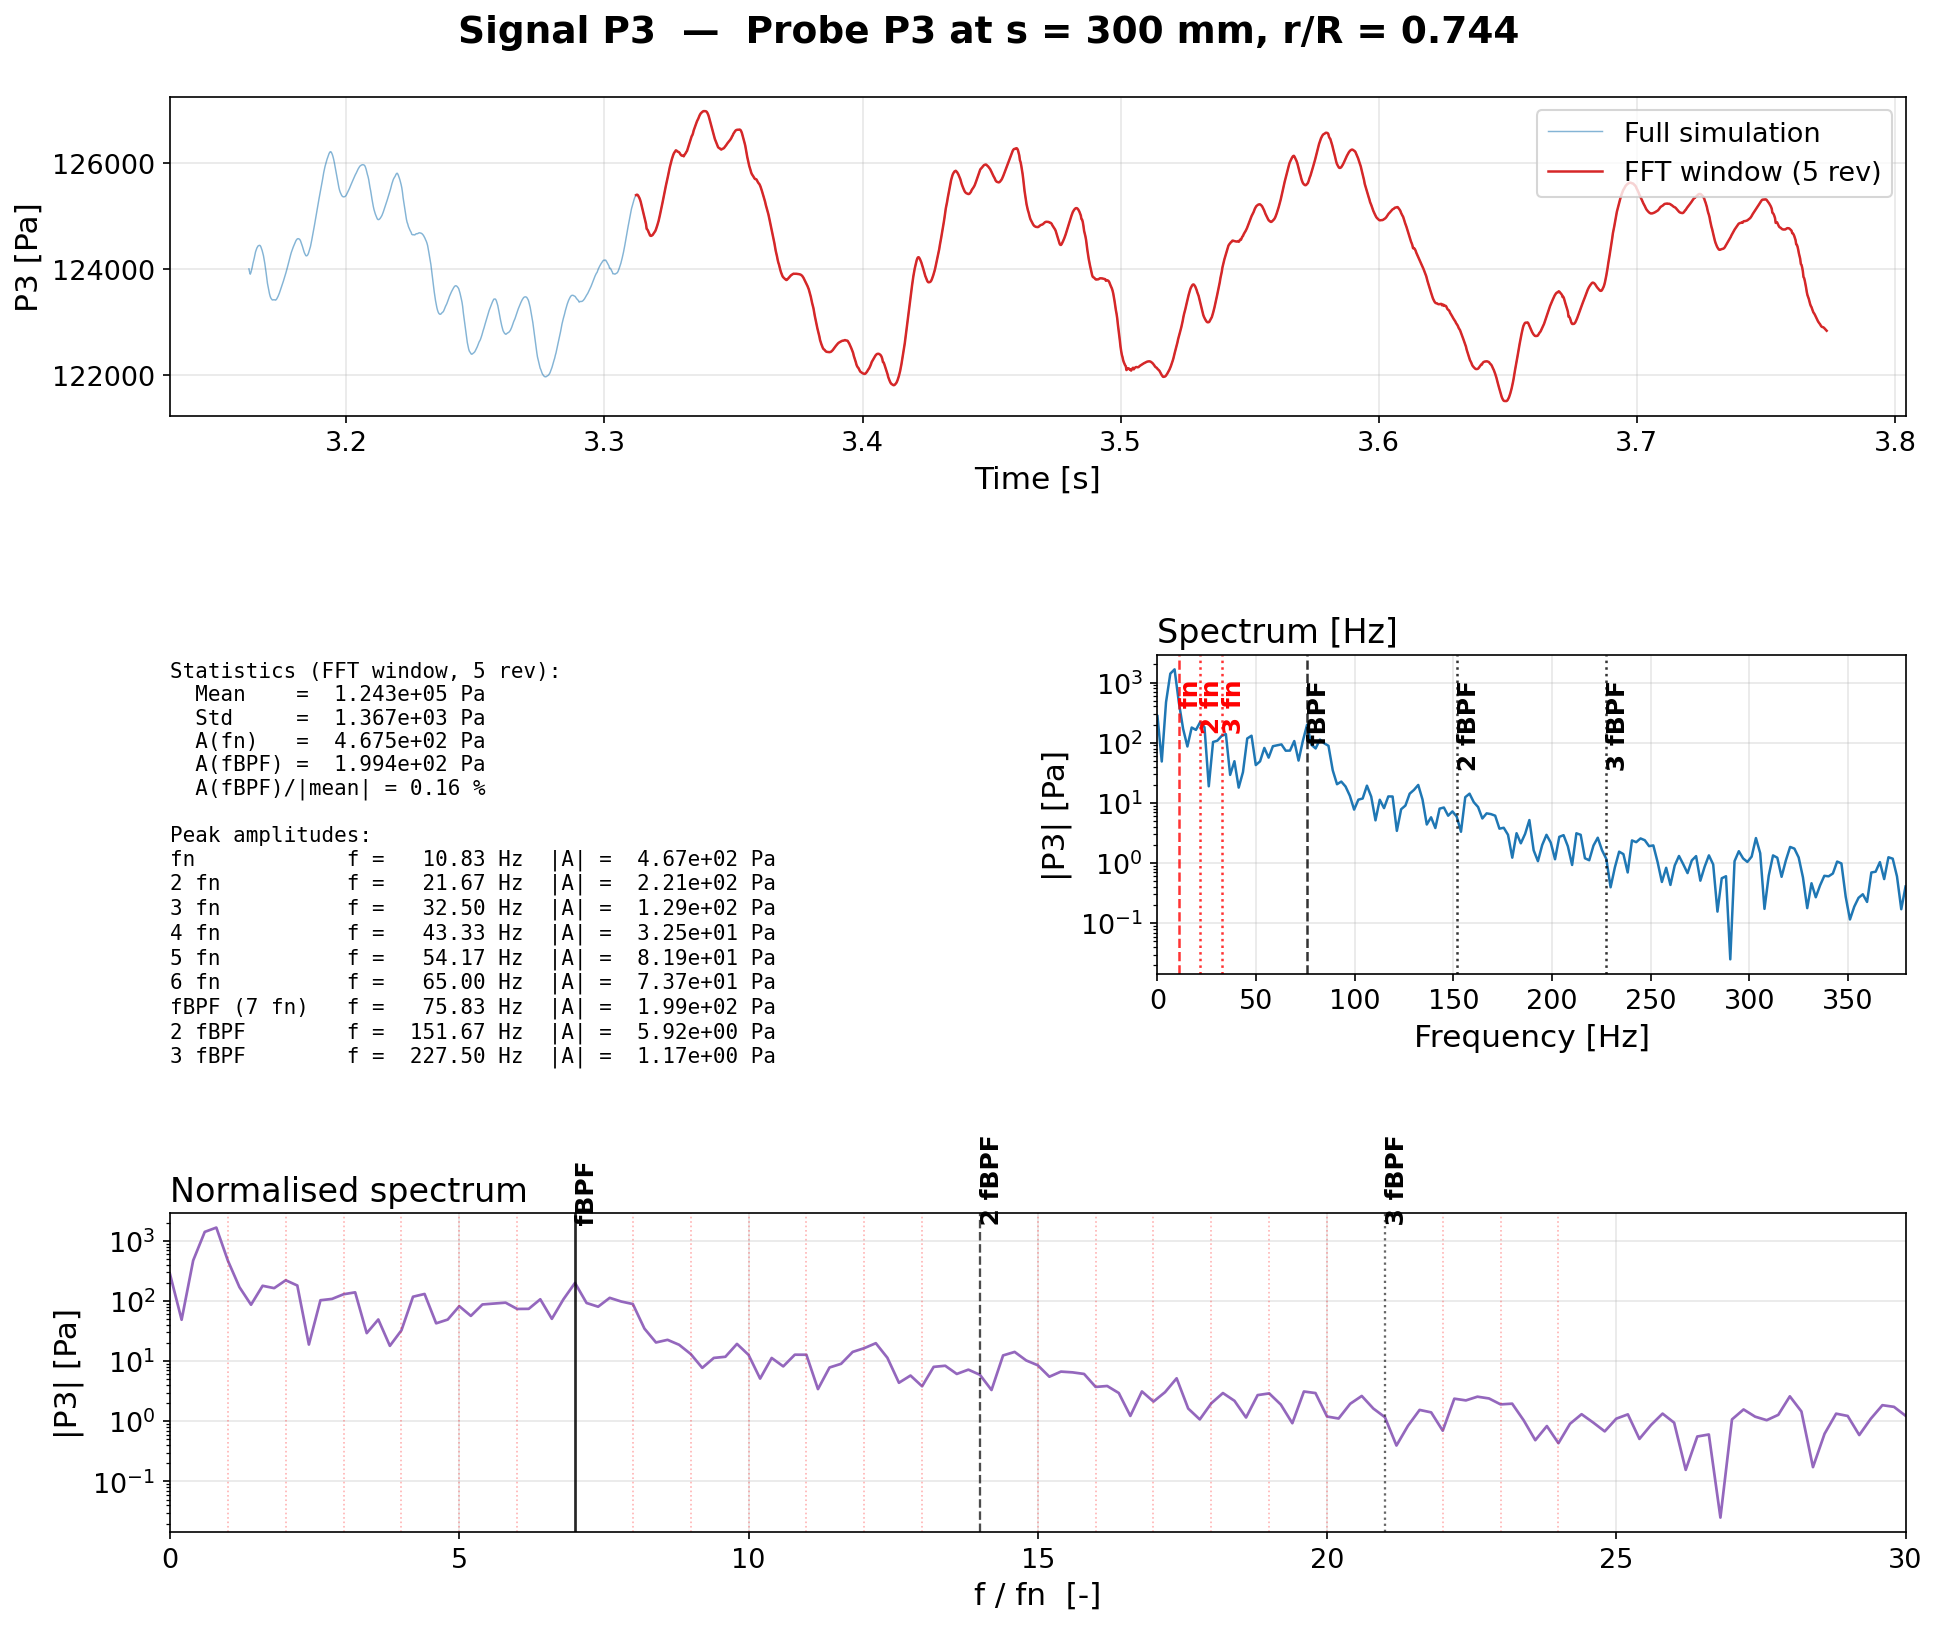
\includegraphics[width=0.95\linewidth]{Figures/FFT/signal_P3.png}
\caption{$P_3$ — Wall probe at $s = 300$~mm, $r/R = 0.744$.}
\end{figure}

\begin{figure}[H]\centering
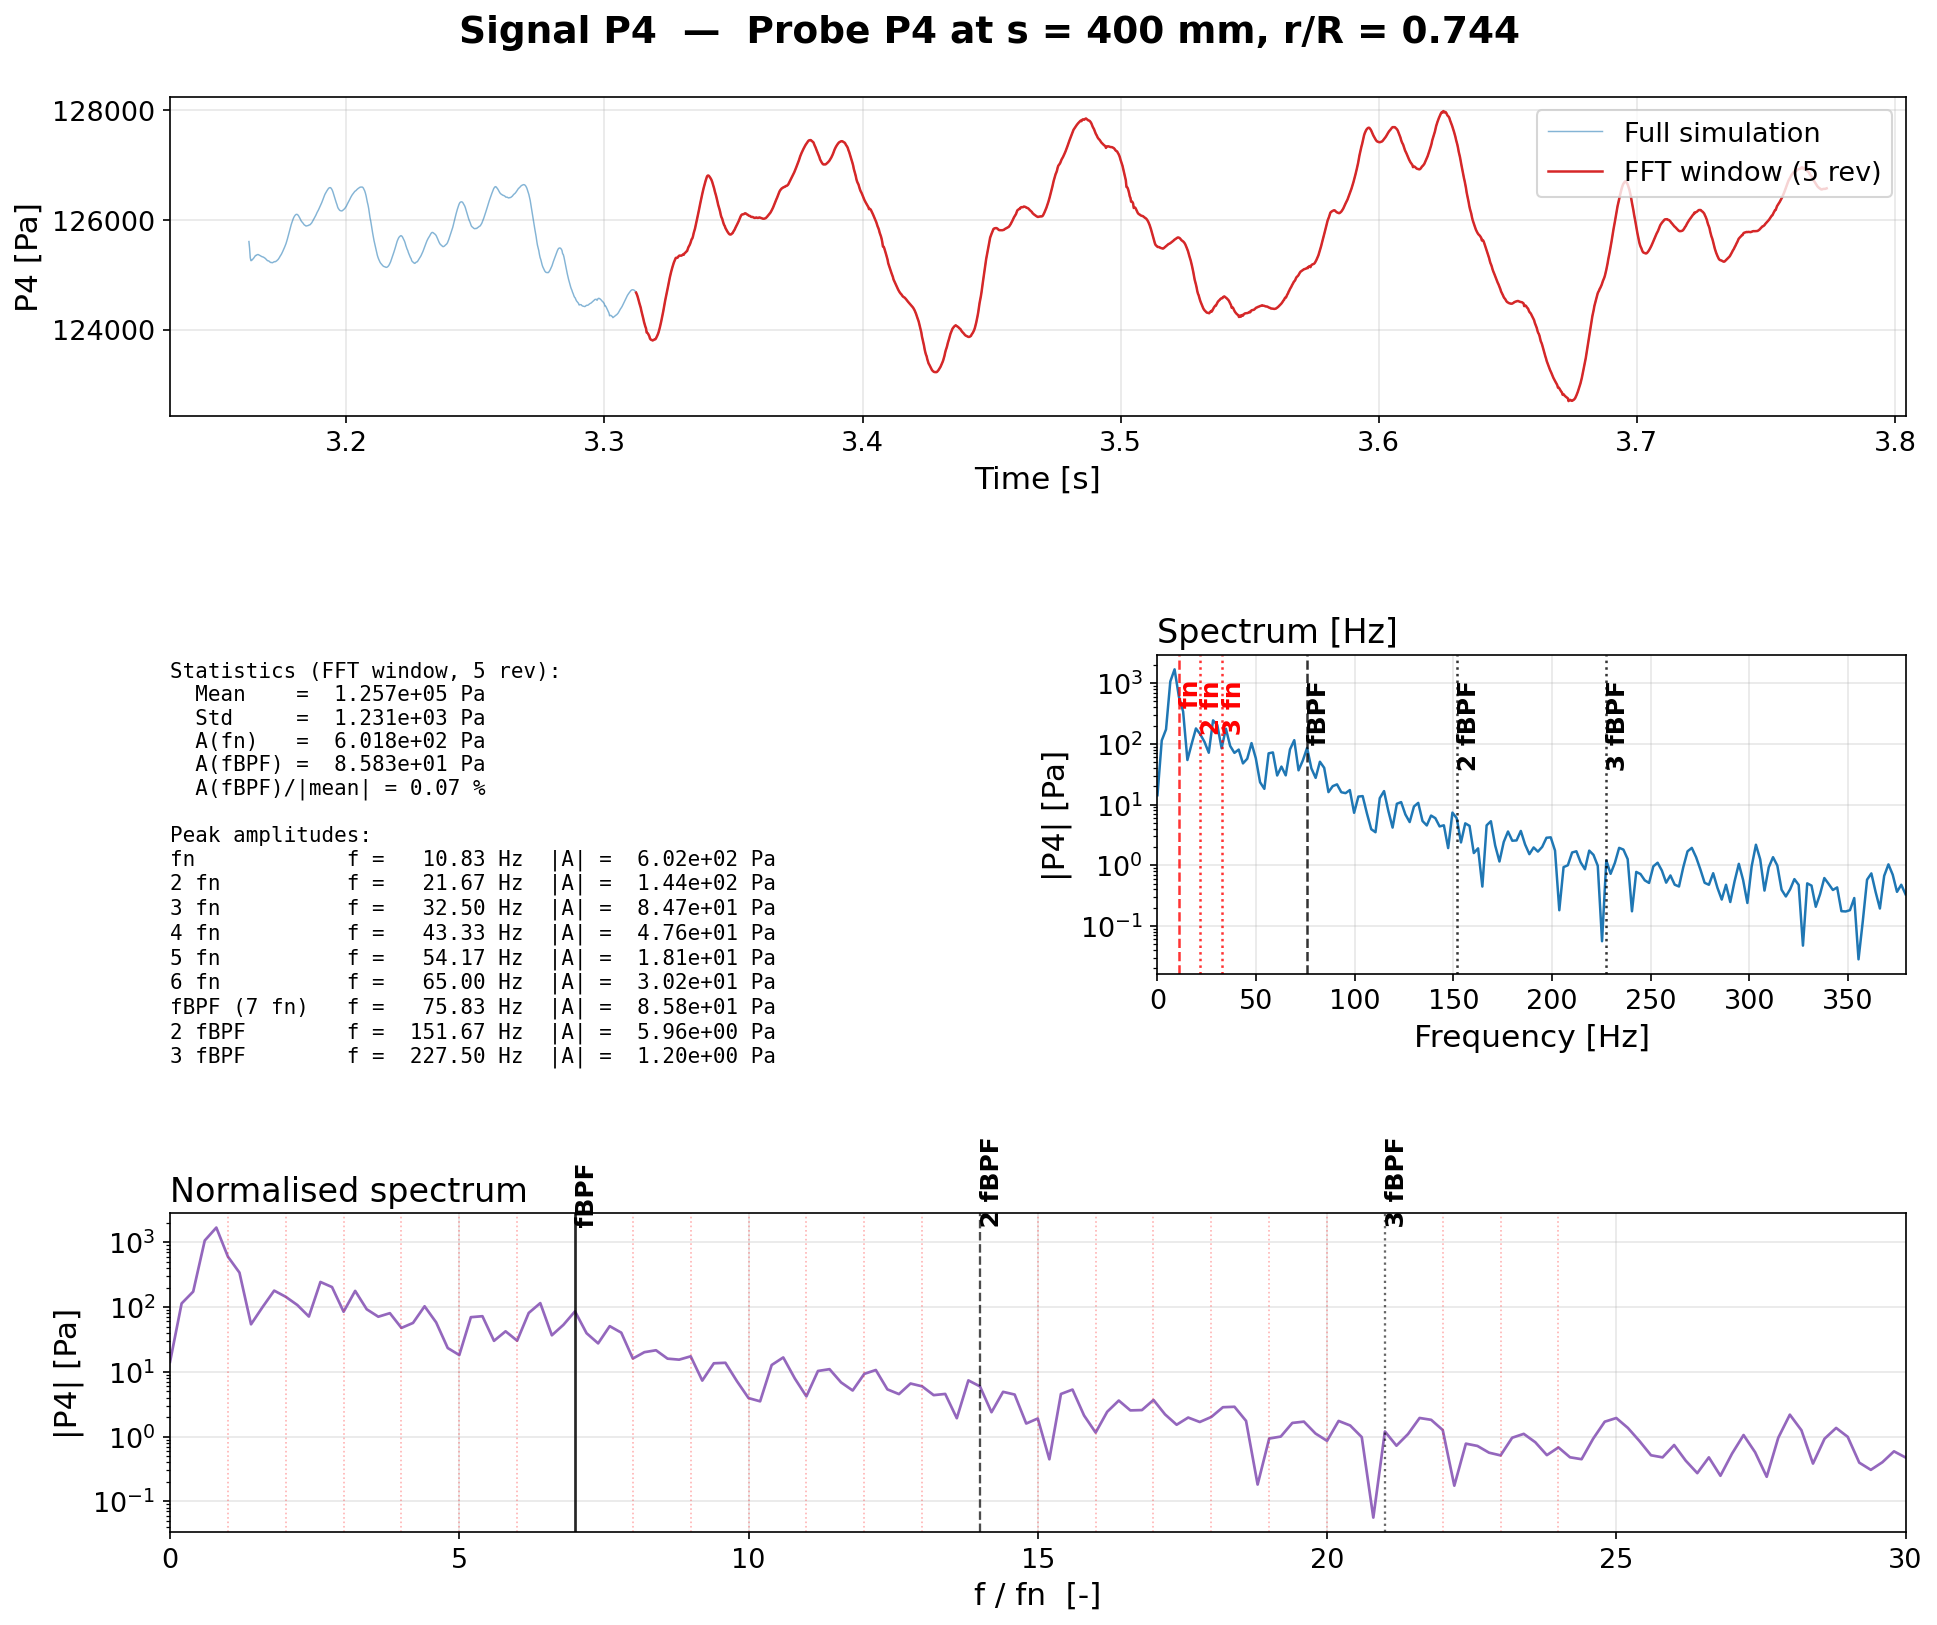
\includegraphics[width=0.95\linewidth]{Figures/FFT/signal_P4.png}
\caption{$P_4$ — Wall probe at $s = 400$~mm, $r/R = 0.744$.}
\end{figure}

\begin{figure}[H]\centering
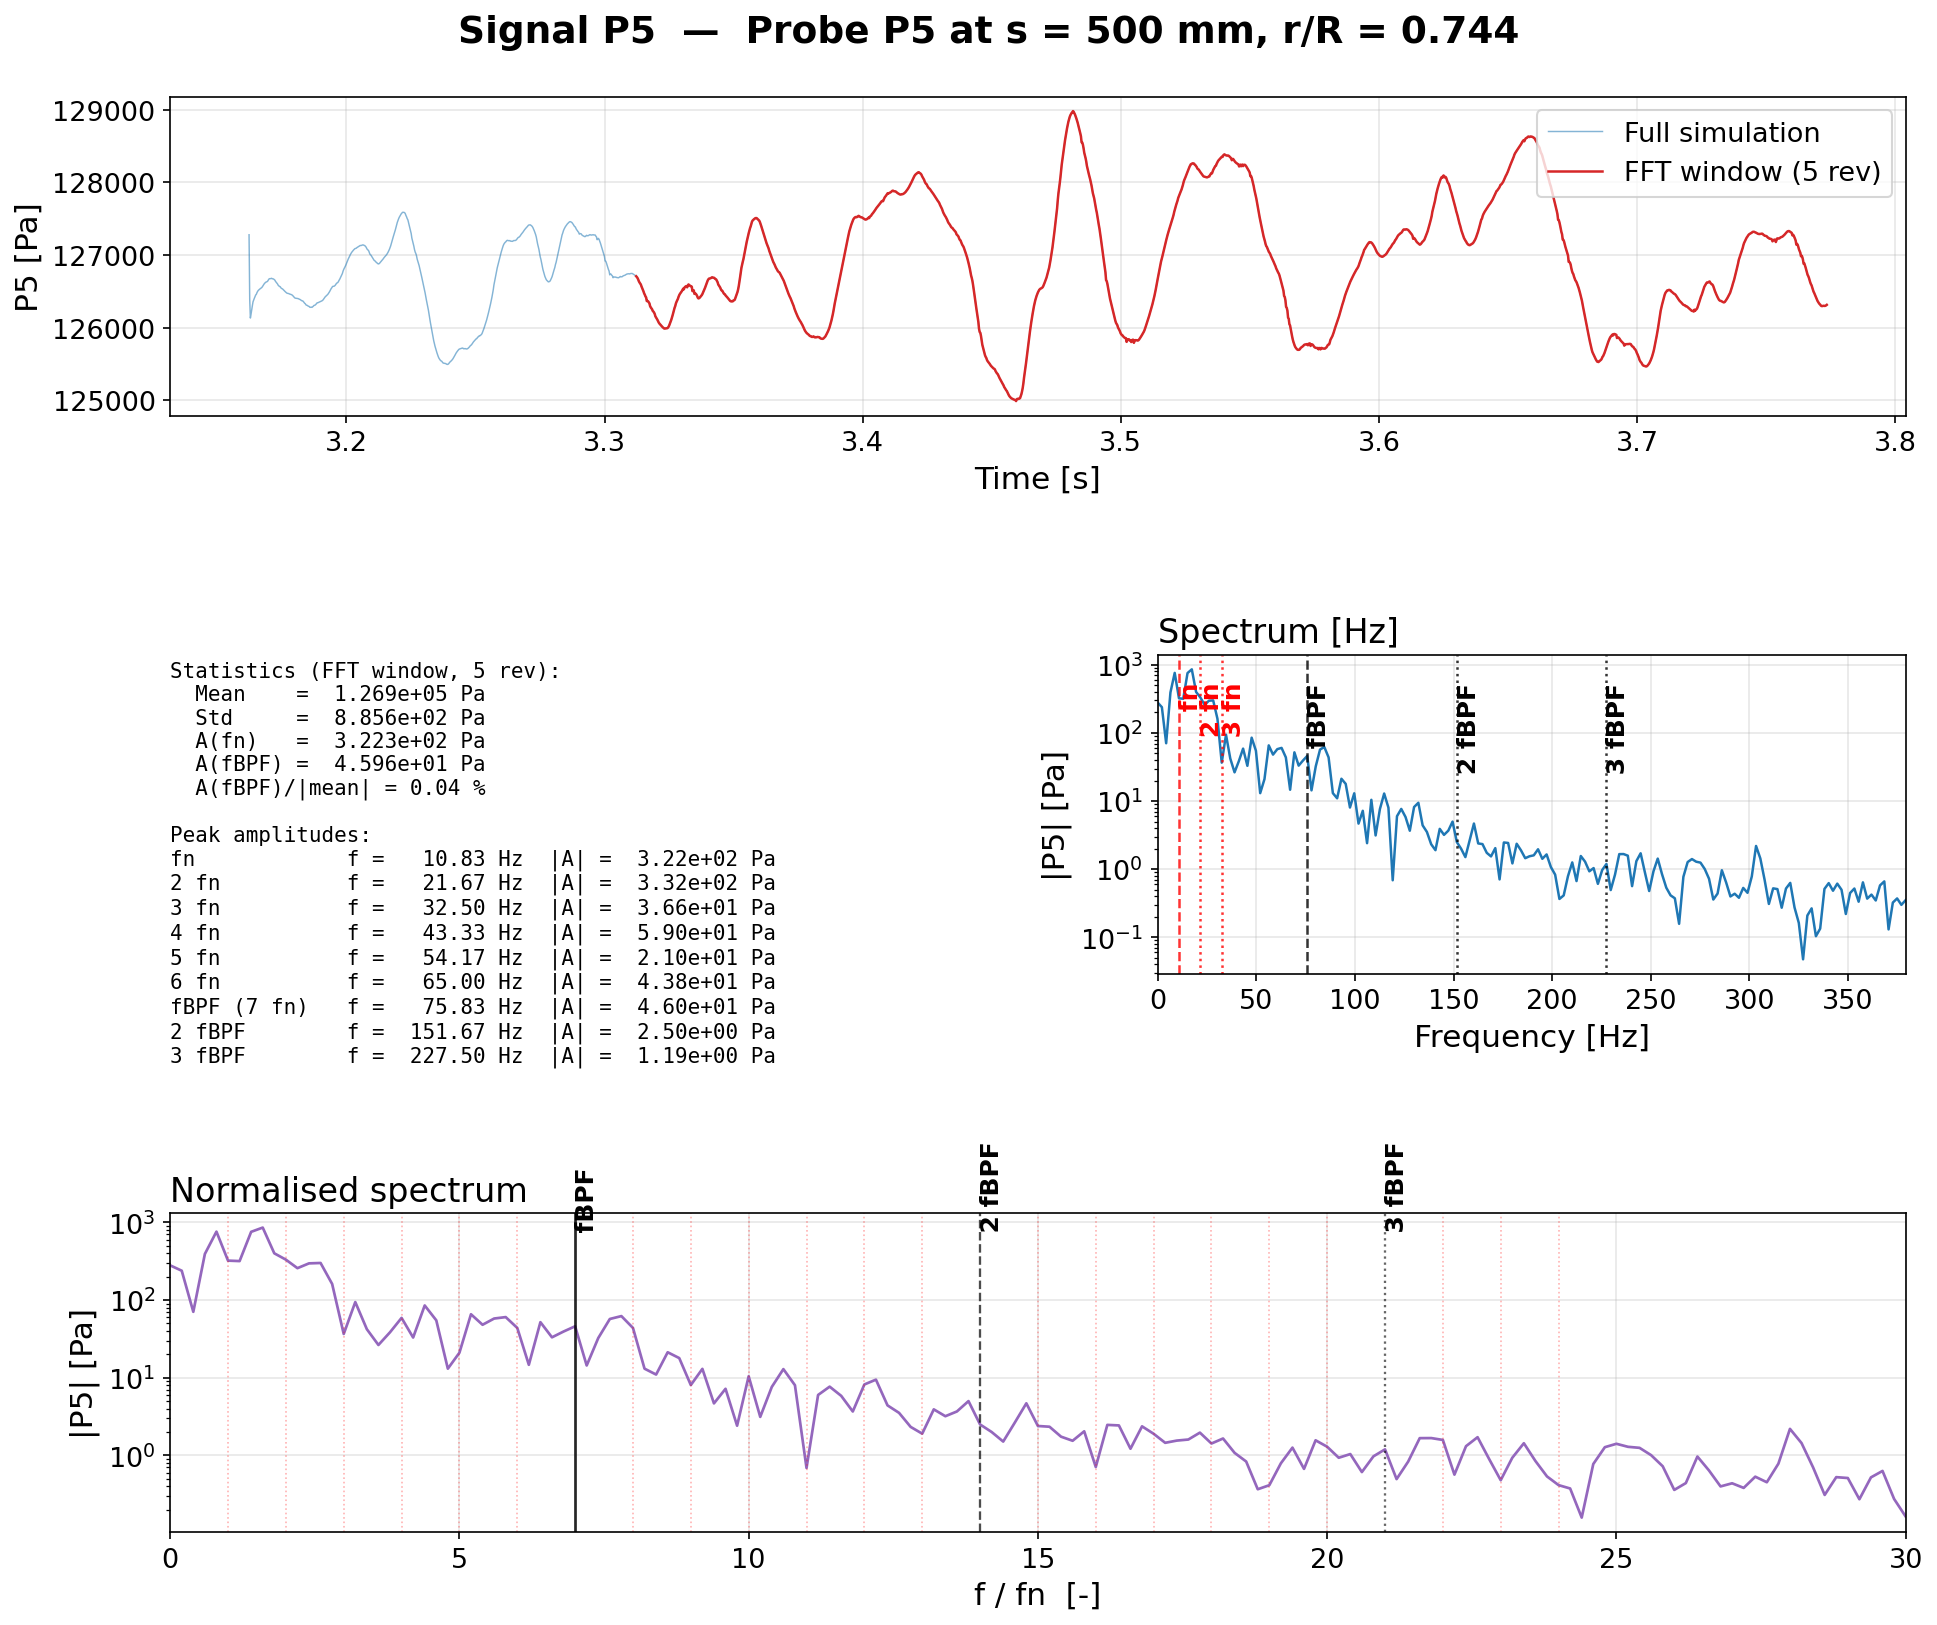
\includegraphics[width=0.95\linewidth]{Figures/FFT/signal_P5.png}
\caption{$P_5$ — Wall probe at $s = 500$~mm, $r/R = 0.744$.}
\end{figure}
